\chapter{Zaimplementowane elementy maszyny wirtualnej}
\label{cha:maszyna}

Maszyna wirtualna jest warstwą abstrakcji uruchamianą pod kontrolą pewnego systemu operacyjnego.
Powinna ona emulować fizyczny procesor w taki sam sposób niezależnie od systemu operacyjnego czy fizycznej architektury, na jakiej została uruchomiona.
Dzięki temu możliwe jest uruchomienie tego samego kodu, nazywanego kodem pośrednim, przystosowanego do architektury maszyny wirtualnej, pod kontrolą różnych systemów operacyjnych i na różnych architekturach sprzętowych.

Wśród funkcjonalności wirtualnego procesa, które powinna implementować maszyna wirtualna dowolnego języka można wymienić:
\begin{itemize}
\item struktury danych, przy pomocy których opisane są instrukcje i ich argumenty;
\item stos, wykorzystywany do wywołań funkcji;
\item wskaźnik kolejnej instrukcji do wykonania;
\item interpreter kodu pośredniego, pobierający kolejną instrukcję do wykonania, dekodujący jej argumenty i wykonujący ją.
\end{itemize}

W rozdziale wymieniono elementy maszyny wirtualnej Erlanga, które zaimplementowane ramach w pracy, tak aby powyższy zbiór funkcjonalności zapewniał możliwość wykonywania kodu modułów skompilowanych przy użyciu kompilatora Erlanga w wersji R16.
Opis poszczególnych elementów zawiera wyjaśnienie ich sposobu działania, ich roli w maszynie wirtualnej, a także porównania
funkcjonalności do maszyny wirtualnej BEAM.

Wszystkie opisywane funkcjonalności zostały zaimplementowane w języku C, podobnie jak jest to w przypadku maszyny wirtualnej BEAM.

%---------------------------------------------------------------------------
\section{Moduł ładujący kod (\emph{loader})}
\label{sec:maszynaLoader}

Moduł opisany w niniejszym podrozdziale został zaimplementowany w pliku źródłowym \texttt{beam\_load.c}.

Podstawowym zadaniem \emph{loadera} jest wykonanie zestawu operacji, po których będzie możliwe wykonanie kodu programu, zawartego w pliku będącym efektem kompilacji modułu w języku Erlang, z~poziomu interpretera kodu pośredniego w maszynie wirtualnej.
W maszynie BEAM źródłem plików binarnych może być system plików systemu operacyjnego lub inny węzeł Erlanga znajdujący się w tym samym klastrze. Aby pliki te mogły być wykonywane na maszynie zaimplementowanej w ramach pracy, która nie obsługuje ani systemu plików ani protokołu klastrowania, muszą one ulec przetworzeniu i zostać wkompilowane w kod maszyny wirtualnej. Dokonywane jest to za pomocą narzędzia opisanego w~dodatku \ref{cha:builder}.

Zawartość pliku, który poddawany jest przetwarzaniu w module została szczegółowo opisana w dodatku \ref{cha:erlangKompilacja}, który ze względu na brak oficjalnej dokumentacji powstał na potrzeby niniejszej pracy.

Aby możliwe było wykonywanie kodu pośredniego przez maszynę wirtualną, konieczne jest wykonanie następujących kroków:
\begin{itemize}
\item załadowanie lokalnej tablicy atomów (fragment \texttt{Atom}) do globalnej tablicy atomów (por. \ref{sub:maszynaTablicaAtomow});
\item załadowanie lokalnej tablicy eksportowanych funkcji (fragment \texttt{ExpT}) do globalnej tablicy (por. \ref{sub:maszynaTablicaEksportow});
\item sparsowanie wyrażeń w postaci \emph{External Term Format}, umieszczonych we fragmencie \texttt{LitT} i~umieszczenie ich w pamięci o globalnym dostępie (globalnej stercie);
\item wyszukanie w globalnej tablicy eksportów funkcji zewnętrznych używanych przez moduł (fragment \texttt{ImpT});
\item podstawienie wyrażeń rozpoznawanych globalnie (por. \ref{sec:maszynaTypy}) za wyrażenia lokalne, opisane w podrozdziale \ref{sec:opsTypes}, we fragmencie \texttt{Code}. Do rozważanych wyrażeń należą: atomy, etykiety lokalnych funkcji, odnośniki do funkcji znajdujących się w innych modułach oraz wyrażenia umieszczone na globalnej stercie;
\item podstawienie za numery operacji z sekcji \texttt{Code}, opisane w podrozdziale \ref{sec:opsOps}), wskaźników do odpowiedniej sekcji interpretera kodu maszynowego wykonującemu daną instrukcję (por. \ref{sec:maszynaInterpreter}).
\end{itemize}

\emph{Loader} maszyny wirtualnej BEAM wykonuje jeszcze jeden bardzo istotny krok, którego nie wykonuje maszyna zaimplementowana w pracy. Jest nim zastosowanie gramatyki modyfikującej w bardzo istotny sposób kod maszynowy zawarty w pliku binarnym. Gramatykę tę można znaleźć w pliku \texttt{ops.tab} w kodzie źródłowym maszyny BEAM. Wynikowy zestaw instrukcji, odpowiadający instrukcjom faktycznie interpretowanym przez BEAM, jest dużo bardziej obszerny od zestawu który może zostać wygenerowany przez kompilator i został opisany w dodatku \ref{cha:operacjeBeam}. Motywacją do zmiany kodu maszynowego w~ten sposób jest m.in. optymalizacja czasu wykonania często występujących po sobie operacji. W przeciwieństwie do oryginalnej maszyny wirtualnej, interpreter zawarty w niniejszej maszynie wirtualnej dokonuje bezpośredniej interpretacji opkodów, które znajdują się w pliku binarnym z kodem pośrednim.

%---------------------------------------------------------------------------
\section{Tablice}
\label{sec:maszynaTablice}

Tablice opisane w tym podrozdziale zostały zaimplementowane w plikach \texttt{hash.c}, \texttt{index.c}, \texttt{atom.c} oraz \texttt{export.c}.

Biorąc pod uwagę modułowy charakter aplikacji napisanych w języku Erlang, maszyna wirtualna musi posiadać pewien mechanizm pozwalający na utrzymywanie globalnego stanu systemu w zależności od aktualnie załadowanych modułów.

Strukturą danych przeznaczoną do tego celu jest tablica z haszowaniem wspomagana przez tablicę indeksów. Połączenie tych dwóch struktur umożliwia wstawienie nowego elementu oraz sprawdzenie jego indeksu w czasie stałym (konieczne jest wyliczenie skrótu). W takim samym czasie (nie jest do tego jednak konieczne wyliczanie skrótu) możliwe jest znalezienie obiektu znając jego indeks. Co więcej, w~reprezentacji kodu maszynowego posługiwanie się indeksami obiektów trywializuje ich porównywanie czy pobieranie ich wartości w trakcie jego wykonywania.

Wybór takiej struktury danych ma więc charakter optymalizacyjny. W maszynie wirtualnej tablicowanymi obiektami są: \textbf{atomy} i \textbf{eksportowane funkcje}. Maszyna wirtualna BEAM dodatkowo tablicuje również \textbf{moduły}, gdzie przechowywane są informacje o wskaźnikach do początku kodu modułu w dwóch wersjach: nowej i starej, które mogą działać w maszynie wirtualnej niezależnie od siebie. Ponieważ jednak maszyna rozważana w pracy w obecnej fazie rozwoju nie zapewnia możliwości dynamicznego ładowania modułów, implementacja tej struktury nie było konieczne.

Na rysunku \ref{fig:atomtable} przedstawiono sposób w jaki wewnątrz maszyny wirtualnej przechowywane są stablicowane dane.  Przykład ten dotyczy dwuelementowej tablicy atomów, które były do niej wstawiane w~kolejności: \texttt{erlang}, \texttt{+}. Strzałki na diagramie reprezentują przechowywanie wskaźników na struktury atomów przez tablice: z haszowaniem i indeksów.

\begin{figure}[h]
\centerline{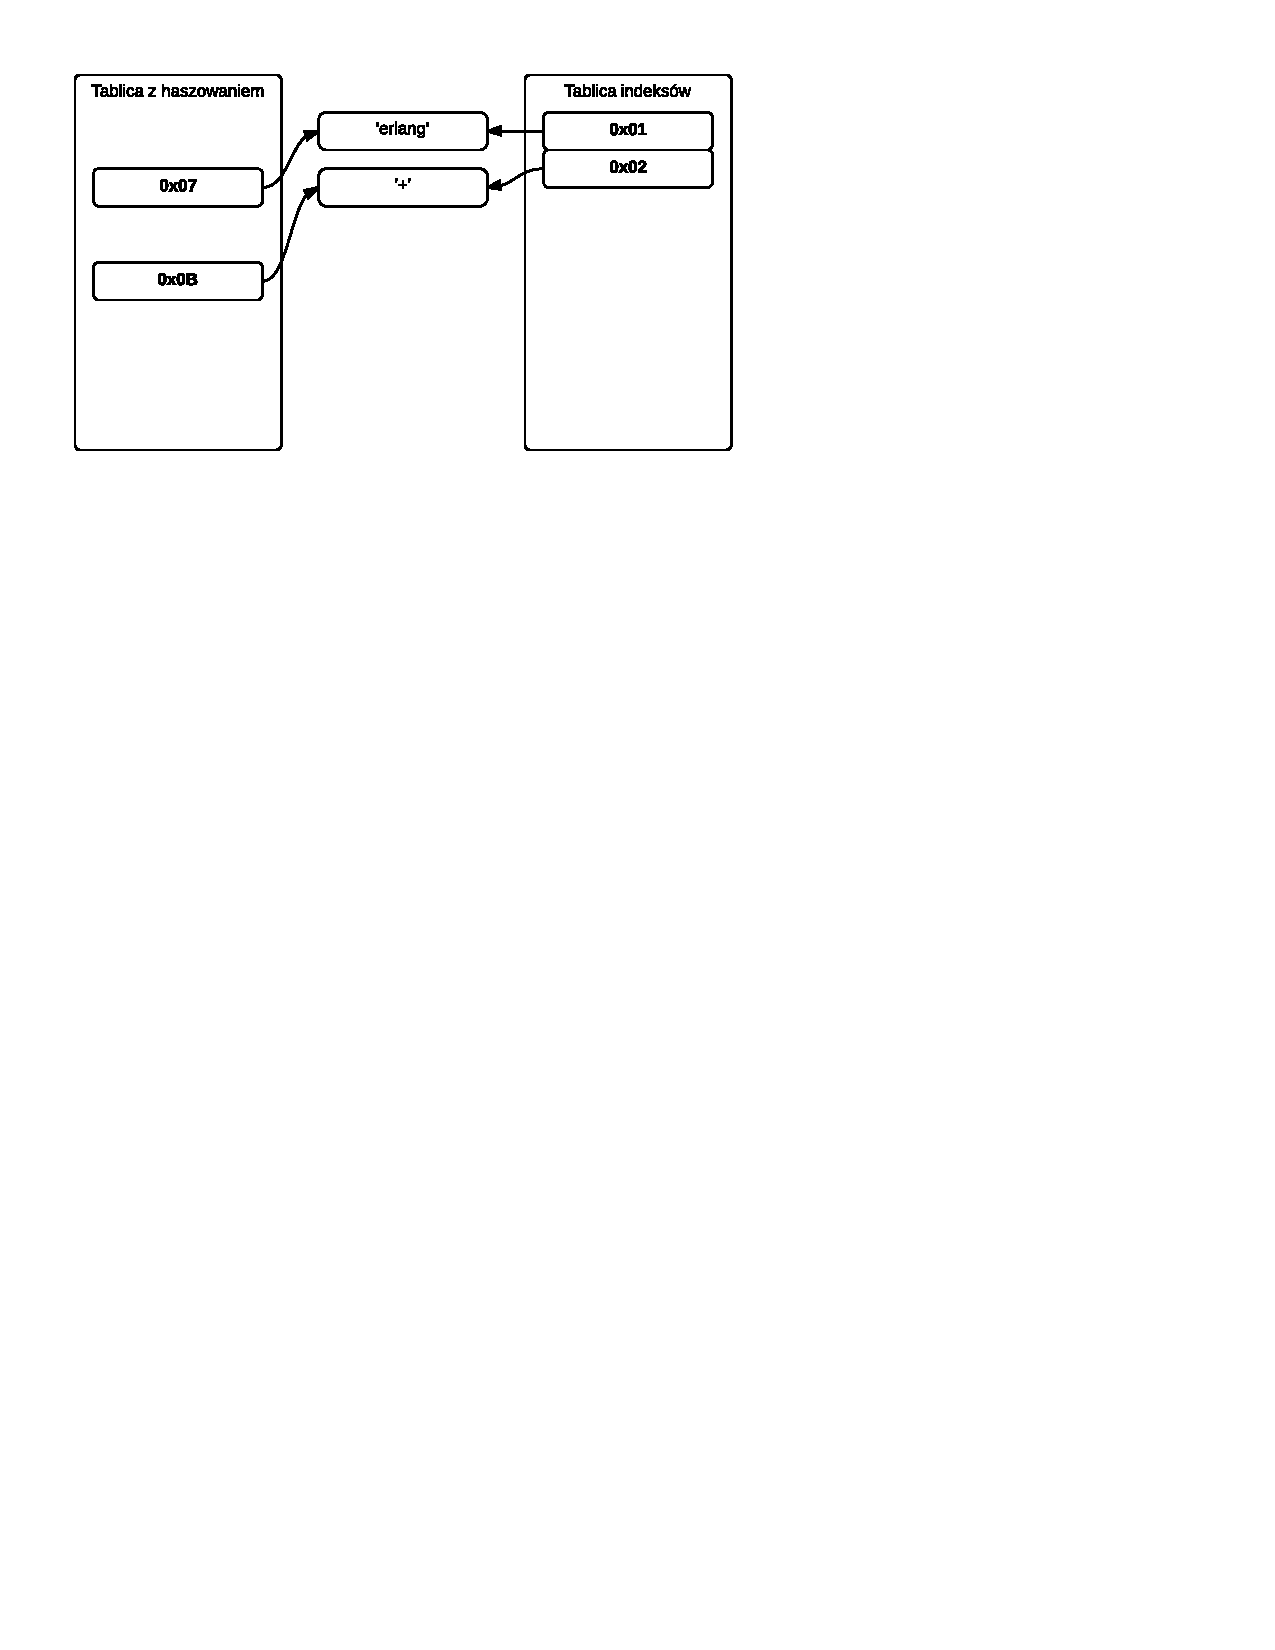
\includegraphics[scale=1, clip, trim=0 200mm 90mm 0]{atom_table}}
\caption{Przykład przechowywania danych stablicowanych danych wewnątrz maszyny wirtualnej.}
\label{fig:atomtable}
\end{figure}

W maszynie BEAM, w przypadku uruchomionych dużych systemów, powyższe struktury danych mogą zawierać bardzo dużą liczbę elementów, nawet rzędu kilkudziesięciu tysięcy. Zupełnie inaczej sytuacja wygląda w niniejszej maszynie wirtualnej ze względu na jej przeznaczenie, którym są systemy wbudowane i wynikające z tego restrykcyjne limity dostępnej pamięci RAM. Rozmiary tablic nie powinny zatem przekraczać liczby elementów wyrażonej w setkach atomów czy funkcji eksportowanych. Niemniej jednak, ze względu na możliwość uruchomienia systemu FreeRTOS na mikrokontrolerach o różnych parametrach, pozostawiono możliwość zdefiniowania maksymalnej liczby elementów, jakie mogą zostać wstawione do tablic. Zaimplementowano również mechanizmy automatycznego rozszerzania tablic wraz ze wzrostem liczby elementów, w celu optymalizacji pamięci zajmowanej przez tablice.

Ważną cechą charakterystyczną tablic w maszynie wirtualnej jest również fakt, że raz wstawionego do nich obiektu nie można z niej usunąć. W kontekście maszyny wirtualnej rozważanej w pracy ta cecha nie ma większego znaczenia, gdyż obecnie nie umożliwia ona dynamicznego ładowania modułów po jej uruchomieniu. Jednak w przypadku maszyny BEAM nie należy zapominać o tej cesze np. w sytuacji, gdy program dynamicznie generuje atomy. Tablica atomów w BEAM może przechowywać aż 1048576 atomów, należy jednak mieć na uwadze to, że próba dodania atomu do pełnej już tablicy zakończy się zakończeniem procesu maszyny wirtualnej.

%---------------------------------------------------------------------------
\subsection{Tablica atomów}
\label{sub:maszynaTablicaAtomow}

Funkcja skrótu dla atomów (ich reprezentacji w postaci napisu) używana w maszynie wirtualnej to \emph{hashpjw} \cite{Aho1986}. Jest to funkcja o bardzo dobrym rozkładzie wartości skrótu dla napisów, jednak wartość zwracana przez oryginalną funkcję jest 32-bitowa.

W celu ograniczenia pamięci zajmowanej przez tablice w maszynie wirtualnej rozważanej w pracy, funkcja haszująca została zmodyfikowana tak, aby zwracała wynik 8-bitowy. Ze względu na duże różnice w rozmiarach tablic pomiędzy rozważaną maszyną a BEAM zmniejszenie długości skrótu zwracanego z funkcji haszującej nie będzie miało wpływu na liczbę kolizji w tablicy z haszowaniem. 

Źródłem atomów w tablicy są atomy zdefiniowane w samej maszynie wirtualnej oraz atomy pochodzące z ładowanych modułów. Atomy zdefiniowane ładowane są do tablicy w trakcie uruchamiania maszyny wirtualnej w określonej kolejności, co za tym idzie atomy te mają z góry ustalony i znany indeks, co jest wykorzystywane np. przy definicji funkcji wbudowanych w maszynę wirtualną (por. \ref{sec:maszynaBIF}). Z kolei indeksy atomów, które pochodzą z ładowanych modułów, a nie zostały wcześniej zdefiniowane, przydzielane są w~kolejności ładowania modułów i występowania atomów w tablicach atomów modułów. Równość dwóch atomów oznacza zawsze równość ich indeksów w globalnej tablicy atomów i na odwrót, niezależnie od źródła ich pochodzenia ani momentu załadowania modułu do maszyny wirtualnej.

%---------------------------------------------------------------------------
\subsection{Tablica eksportowanych funkcji}
\label{sub:maszynaTablicaEksportow}

Funkcja skrótu dla eksportowanych funkcji ma wartość $M \cdot F+A$, gdzie $M$ to indeks w tablicy atomów dla nazwy modułu z którego eksportowana jest funkcja, $F$ to indeks w tablicy atomów dla nazwy eksportowanej funkcji, a $A$ to arność tej funkcji.

Wpisy w tablicy eksportowanych funkcji pochodzą z modułów załadowanych do maszyny wirtualnej, dla funkcji które zostały zdefiniowane w lokalnej tablicy eksportów dla danego modułu. W takiej sytuacji w tablicy eksportów przechowywany jest wskaźnik na miejsce w pamięci, w którym znajduje się pierwsza instrukcja funkcji. Interpreter, wykonując kod używa indeksu do odczytania adresu tej instrukcji, a następnie wykonuje skok do tego miejsca pamięci i kontynuuje wykonywanie kodu, po uprzednim zapisaniu adresu powrotu.

Elementy tablicy mogą pochodzić również z wbudowanych funkcji (por. \ref{sec:maszynaBIF}). W tym przypadku, tablica eksportów zawiera wskaźnik do funkcji w języku C, zaimplementowanej jako część maszyny wirtualnej, która zostanie wykonana przez interpreter.

Ponieważ równość indeksów w tablicy eksportów jest równoważna z równością trójek $\lbrace\text{moduł},\text{funkcja},\text{arność}\rbrace$, w sytuacji dynamicznej podmiany kodu nie jest konieczna zmiana indeksu w załadowanym do pamięci kodzie maszynowym, a tylko odpowiednia zmiana struktury znajdującej się pod tym indeksem.

%---------------------------------------------------------------------------
\section{Typy danych}
\label{sec:maszynaTypy}

Erlang jest językiem programowania o dynamicznym, lecz silnym typowaniu. Oznacza to, że każda zmienna, po przypisaniu do niej wartości ma ustalony konkretny typ danych, którego nie można zmienić. Niemożliwe jest również rzutowanie zmiennej na innych typ danych - konwersja do innego typu musi zostać wykonana jawnie a nowa zmienna zajmuje w takiej sytuacji inne miejsce w~pamięci programu.

Wszystkie wyrażenia rozpoznawane przez interpreter kodu maszynowego Erlanga zapisane są w~postaci wyrażenia takiego samego typu, z punktu widzenia języka C, o długości równej słowu maszynowemu dla danej architektury.
W celu rozróżnienia typów zmiennych w pamięci programu, w maszynie wirtualnej wprowadzony został mechanizm \textbf{tagowania}, czyli oznaczania w różny sposób zmiennych w~pamięci, w~zależności od ich typu. Mechanizm ten został zaprojektowany w taki sposób, aby dodatkowy rozmiar w pamięci przeznaczony dla typu był jak najmniejszy. Sposób jego działania został przedstawiony w niniejszej sekcji.

\subsection{Wartości bezpośrednie a pośrednie}
\label{sub:typyTypy}

Podstawowy podział typów danych wewnątrz maszyny wirtualnej Erlanga wynika ze względu na sposób dostępu do danych. 

Jeżeli dana może zostać przechowana na odpowiednio małym obszarze pamięci, czyli w jednym słowie maszynowym (w przypadku niniejszej maszyny są to 32 bity) z uwzględnieniem tagu oznaczającego typ to dane tego typu nazywane są wartościami bezpośrednimi (\textbf{IMMED}). Aby dokonać tagowania lub odczytania wartości ze zmiennej tego typu wystarczy wykonać jedną operację przesunięcia bitowego.

Przeciwieństwem danych bezpośrednich są dane pośrednie, które mogą przybrać postać listy (\textbf{CONS}) lub typu opakowanego (\textbf{BOXED}).
Wyrażenia oznaczone tagiem dla jednego z tych typów przechowują fizyczny wskaźnik na miejsce w~pamięci, gdzie znajdują się dla nich właściwe dane.
Przy tagowaniu wskaźników wykorzystany został fakt, że bloki pamięci alokowane przez maszynę wirtualną są zawsze wielokrotnością całego słowa maszynowego.
Co za tym idzie dwa najmniej znaczące bity wskaźnika, na maszynie uruchomionej w architekturze 32-bitowej lub wyższej będą zawsze zerami co można wykorzystać do przechowania dodatkowej, dwubitowej, informacji. W tym wypadku jest to tag rozróżniający wskaźniki na listy od wskaźników na typy opakowane oraz od pozostałych wyrażeń.

Tabela \ref{table:primaryTags} prezentuje sposób tagowania ww. typów danych.
Tagi dla poszczególnych typów danych zostały w zapisie słowa maszynowego pogrubione.

Na przykład do przechowania wskaźnika do pierwszego elementu listy, znajdującego się pod adresem 128, w pamięci zapisane zostane wyrażenie:
$$\texttt{10000000} \vee \texttt{\textbf{01}} = \texttt{00000000 00000000 00000000 100000\textbf{01}}$$

Do odczytania wartości wskaźnika wystarczy więc wyzerowanie dwóch najmniej znaczących bitów wyrażenia:
$$\texttt{00000000 00000000 00000000 100000\textbf{01}} \wedge  \lnot(\texttt{11}) = \texttt{10000000}$$ 

\begin{longtable}{|c|p{4cm}|p{8cm}|}
\hline

Typ danych & Słowo maszynowe (binarnie) & Opis \\
\endfirsthead
\hline

\textbf{IMMED} & \texttt{IIIIIIII IIIIIIII IIIIIIII IIBBTT\textbf{11}} &
\vspace{-8mm}
\begin{itemize}
\item bity \texttt{T} budują konkretny tag (por. \ref{sub:typyImmediates}) typu bezpośredniego;
\item bity \texttt{I} oznaczają wartość przechowywaną przez wyrażenie, która w zależności od rozmiaru tagu może mieć 26 lub 28 bitów;
\item bity \texttt{B} mogą być dwoma najbardziej znaczącymi bitami tagu lub dwoma najmniej znaczącymi bitami przechowywanej wartości, w zależności od typu.
\end{itemize}  
\vspace{-8mm}
\\
\hline
\textbf{CONS} & \texttt{PPPPPPPP PPPPPPPP PPPPPPPP PPPPPP\textbf{01}} &
\vspace{-8mm}
\begin{itemize}
\item bity \texttt{P} są 30 najbardziej znaczącymi bitami wskaźnika do wyrażenia stanowiącego pierwszy element listy, dwa najmniej znaczące bity zawsze będą zerami dlatego mogą zostać nadpisane przez tag.
\end{itemize}  
\vspace{-8mm}
\\
\hline
\textbf{BOXED} & \texttt{PPPPPPPP PPPPPPPP PPPPPPPP PPPPPP\textbf{10}} &
\vspace{-8mm}
\begin{itemize}
\item bity \texttt{P} są 30 najbardziej znaczącymi bitami wskaźnika do nagłówka identyfikujące typ i~rozmiar opakowanych danych, w tym przypadku również dwa najmniej znaczące bity zawsze będą zerami.
\end{itemize}  
\vspace{-8mm}
 \\
\hline
\caption{Rozróżnienie tagów ze względu na sposób dostępu do danych} 
\label{table:primaryTags} \\
\end{longtable}

\subsection{Wartości bezpośrednie}
\label{sub:typyImmediates}

Wartości bezpośrednie (\textbf{IMMED}) mogą być przechowywane przez różne typy danych, dla których przewidziano dodatkowe 2 lub 4 bity na tag. Tabela \ref{table:secondaryImmed} podsumowuje wszystkie zaimplementowane w~maszynie wirtualnej opisywanej w~pracy typy zawierające wartości bezpośrednie.

\begin{longtable}{|c|p{4cm}|p{8cm}|}
\hline

Typ danych & Słowo maszynowe (binarnie) & Opis \\
\endfirsthead
\hline

\textbf{PID} & \texttt{IIIIIIII IIIIIIII IIIIIIII IIII\textbf{0011}} & Wartością przechowywaną przez wyrażenie tego typu jest indeks procesu w tablicy procesów w maszynie wirtualnej (por. \ref{sec:maszynaProcesy}).\\
\hline
\textbf{SMALL\_INT} & \texttt{IIIIIIII IIIIIIII IIIIIIII IIII\textbf{1111}} & Przechowywaną wartością jest liczba całkowita (ze znakiem), którą można zapisać na maksymalnie 28 bitach w pamięci. \\
\hline
\textbf{ATOM} & \texttt{IIIIIIII IIIIIIII IIIIIIII II\textbf{001011}} & Wartością przechowywaną jest indeks atomu w tablicy atomów (por. \ref{sub:maszynaTablicaAtomow}). Dzięki takiemu zapisowi porównanie dwóch dowolnych atomów sprowadza się do porównania dwóch 32-bitowych liczb.  \\
\hline
\textbf{NIL} & \texttt{00000000 00000000 00000000 00\textbf{111011}} & Przechowywaną wartością jest zawsze zero. Wyrażenie to służy do oznaczania końca listy. \\
\hline
\caption{Rozróżnienie tagów dla danych bepośrednich} 
\label{table:secondaryImmed} \\
\end{longtable}

Na przykład atom mający indeks $2_{10} = 10_{2}$ w tablicy atomów w pamięci będzie zapisany w postaci:
$$(\texttt{10} \ll 6) \vee \texttt{\textbf{001011}} = \texttt{00000000 00000000 00000000 10\textbf{001011}}$$

Do odczytania indeksu atomu wystarczy zatem wykonać operację przesunięcia bitowego w prawo:
$$\texttt{00000000 00000000 00000000 10\textbf{001011}} \gg 6 = \texttt{10}$$

\subsection{Listy}
\label{sub:typyLists}

Listy są jednym ze złożonych typów danych obsługiwanych przez język Erlang.
W maszynie wirtualnej zaimplementowane zostały przy użyciu listy jednokierunkowej.
Wyrażenie, które służy np. do przechowywania listy na stosie procesu lub przekazywania jej jako argument do funkcji otagowane jest jako typ \textbf{CONS} (por. \ref{sub:typyTypy}) i zawiera wskaźnik do pierwszego elementu listy. Element listy jest zwykłym wyrażeniem erlangowym, a więc zajmuje jedno słowo maszynowe. Słowem maszynowym następującym po elemencie jest kolejne wyrażenie typu \textbf{CONS}, które zawiera wskaźnik do kolejnego elementu listy. Wyrażenie to może być również typu \textbf{NIL} (por. \ref{sub:typyImmediates}), co oznacza że dany element był ostatnim elementem listy.

W Erlangu nie ma osobnego typu do przechowywania ciągu znaków. Udostępniony lukier składniowy pozwala jednak na posługiwanie się napisami, np. w postaci: \texttt{"hello"}. Wyrażenie tego typu zostanie jednak zinterpretowane jak lista liczb całkowitych, odpowiadającymi kodom ASCII kolejnych liter w napisie. W tym przypadku będzie to następująca lista: \texttt{[104,101,108,108,111]}.

Na rysunku \ref{fig:listonheap} zaprezentowano przykładową stertę procesu Erlanga zawierającą powyższą listę, wraz z wyjaśnieniem typu i wartości zawartych w poszczególnych słowach maszynowych. 
Wyrażenie będące początkiem listy znajduje się w~pierwszym wierszu sterty.
Strzałki na diagramie reprezentują zawieranie wskaźnika do innego miejsca w pamięci przez wyrażenie z którego wychodzą.

\begin{figure}[h]
\centerline{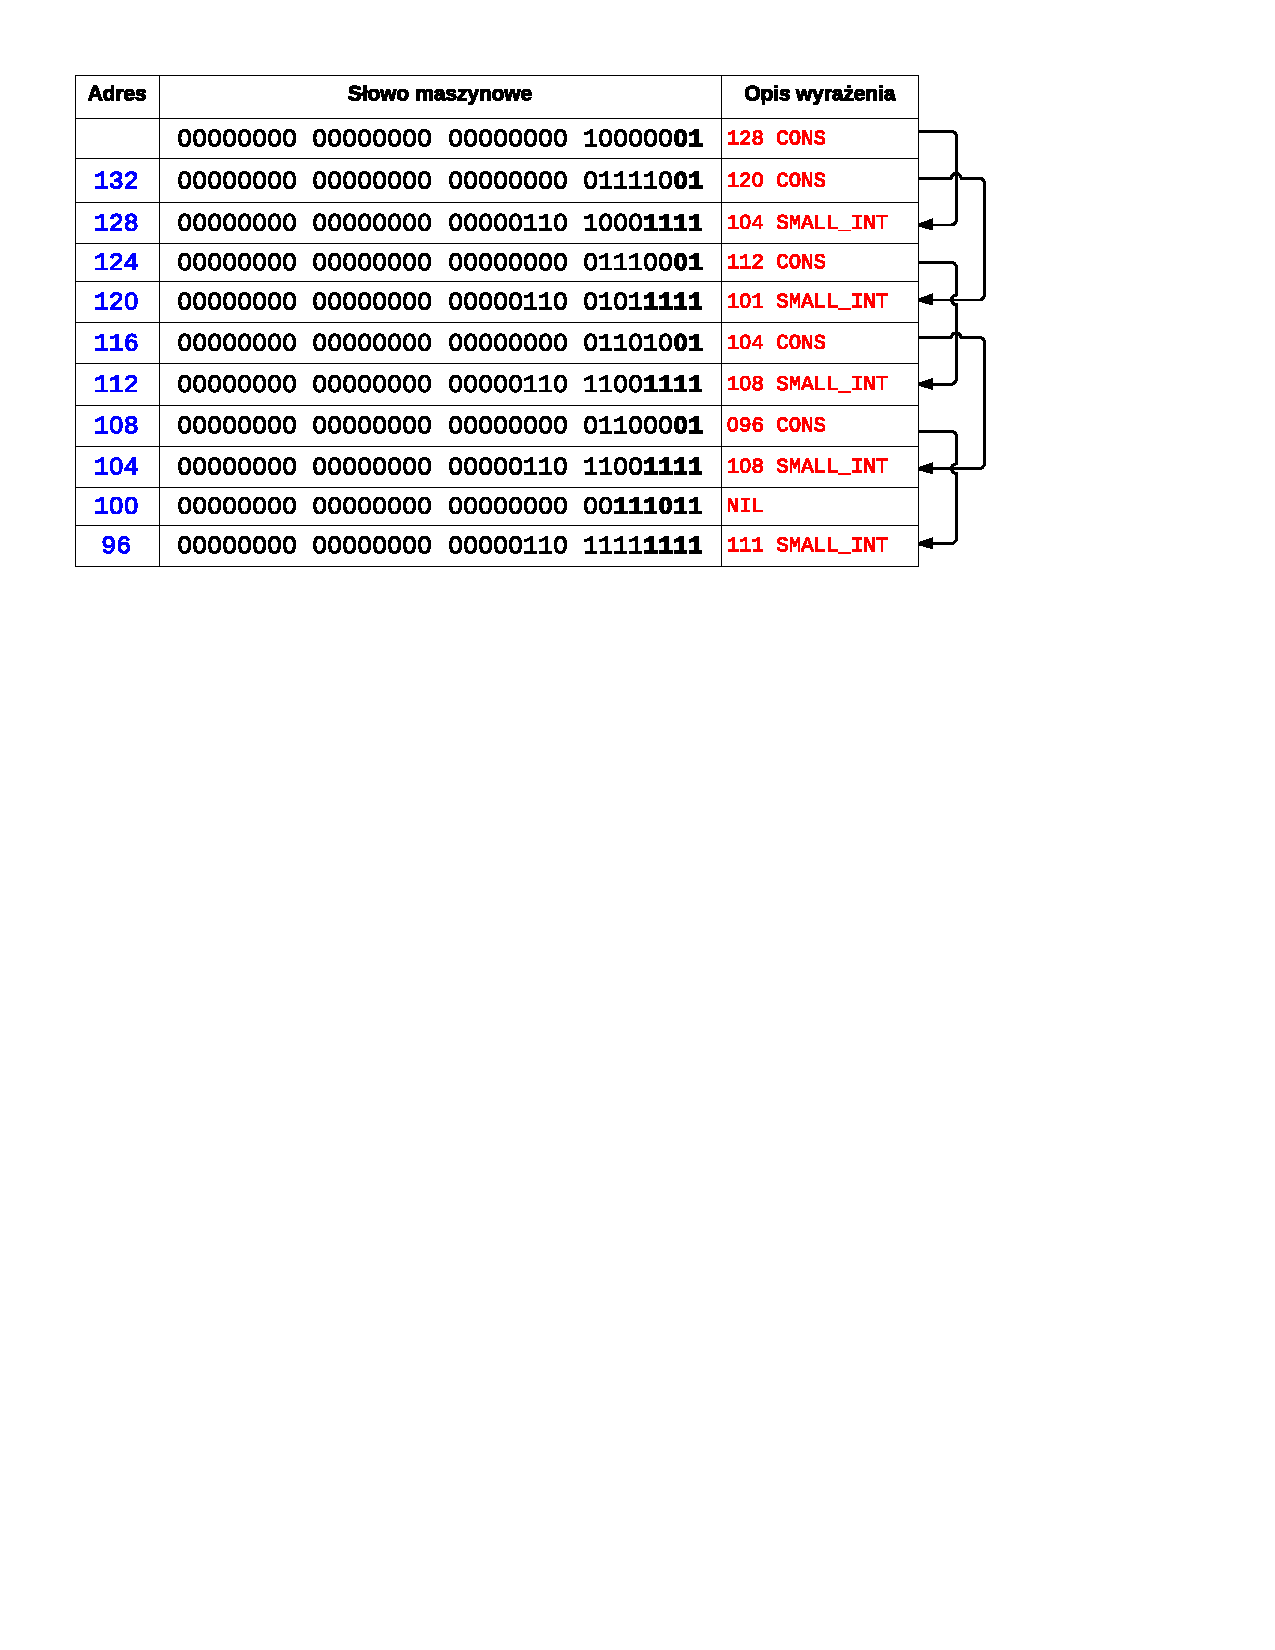
\includegraphics[scale=1, clip, trim=0 180mm 45mm 0]{list_on_heap}}
\caption{Przykład przechowywania listy na stercie procesu}
\label{fig:listonheap}
\end{figure}

Powyższy przykład dobrze ilustruje narzut pamięciowy jaki wprowadza sposób zapisu napisu przy użyciu listy. 
Informacja, która przy użyciu innych języków programowania może być zapisana przy użyciu 5 bajtów w języku Erlang potrzebuje aż 10 słów maszynowych (40 bajtów na architekturze 32-bitowej).
Receptą na tego typu problem, wprowadzoną w maszynie wirtualnej BEAM, jest binarny typ danych. Napis \texttt{"hello"} przy jego użyciu zajmowałby w pamięci 3 słowa maszynowe (nagłówek i~2~słowa przeznaczone na dane).
Typ ten jednak nie został zaimplementowany w obecnej wersji maszyny na system FreeRTOS.  

Jak można zauważyć zarówno złożoność obliczeniowa (dostęp do danych na liście trwa czas liniowy) jak i pamięciowa przy wykorzystaniu tego typu danych jest dość znacząca.

\subsection{Krotki}
\label{sub:typyKrotki}

Kolejnym złożonym typem danym, z którego można korzystać w języku Erlang jest krotka, zajmująca spójny obszar pamięci. Z implementacyjnego punktu widzenia można porównać ją do tablicy zawierającej wyrażenia erlangowe.

Krotka jest jednym z typów opakowanych (\textbf{BOXED}), zatem referencja do niej z poziomu stosu procesu zawiera wskaźnik do nagłówka krotki. Nagłówek, podobnie jak pozostałe wyrażenia zajmuje jedno słowo maszynowe i przechowuje rozmiar krotki w postaci:
$$\texttt{AAAAAAAA AAAAAAAA AAAAAAAA AA\textbf{000000}}$$
gdzie bity \texttt{A} oznaczają rozmiar (arność) krotki. Wyrażenia wchodzące w skład krotki zajmują kolejne, następujące po nagłówku, słowa maszynowe.

Na rysunku \ref{fig:tupleonheap} zaprezentowany został przykład przechowywania danych wewnątrz krotki na stercie procesu, jak w przykładzie na rys. \ref{fig:listonheap}, czyli krotki \texttt{\{104,101,108,108,111\}}.

\begin{figure}[h]
\centerline{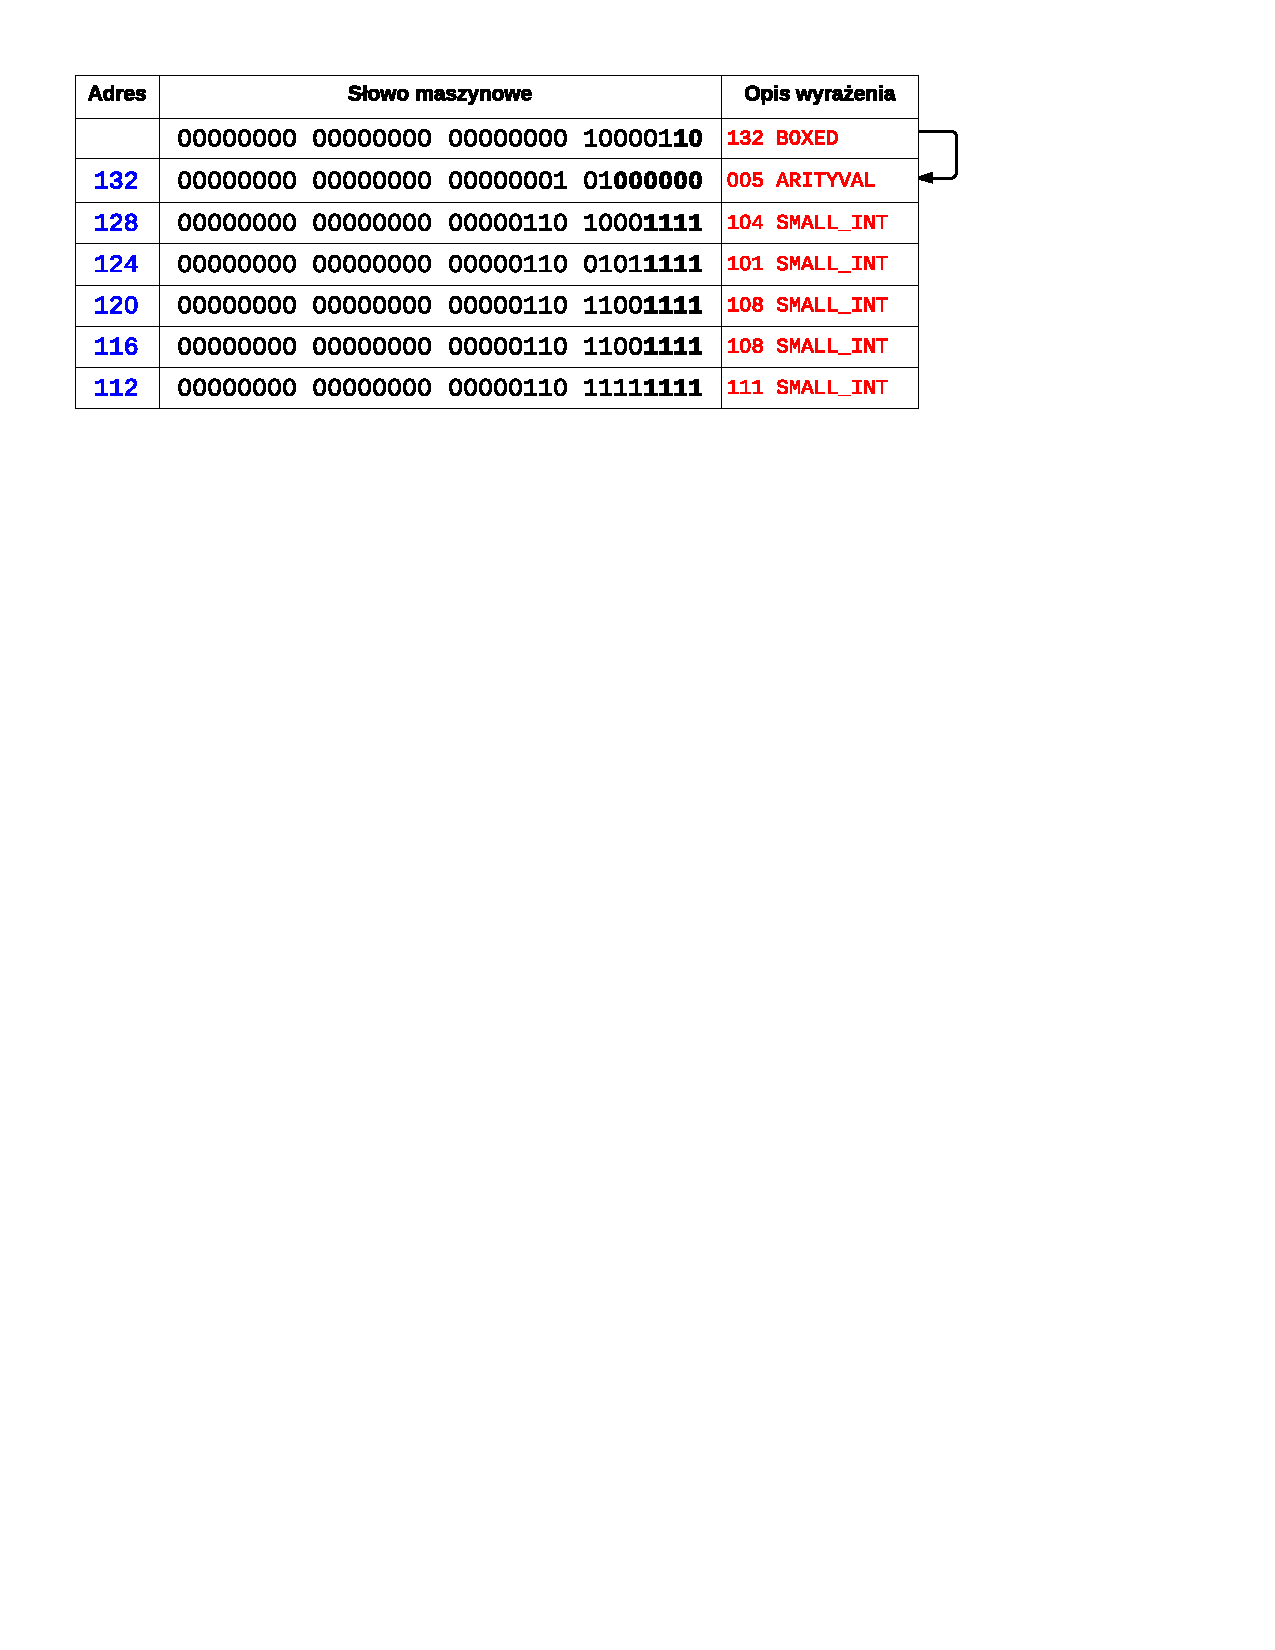
\includegraphics[scale=1, clip, trim=0 210mm 45mm 0]{tuple_on_heap}}
\caption{Przykład przechowywania krotki na stercie procesu}
\label{fig:tupleonheap}
\end{figure}

Ze względu na to, że krotka przechowuje dane w spójnym obszarze pamięci i dostęp do nich odbywa się w czasie stałym, użycie tego typu danych jest dobrym pomysłem w przypadku przechowywania danych tablicowych.

\subsection{Duże liczby}
\label{sub:typyBigs}

Drugim zaimplementowanym, opakowanym typem danych są duże liczby całkowite.
Wszystkie liczby całkowite, które nie mieszczą się w zakresie typu \textbf{SMALL\_INT}, czyli potrzebują do ich zapisania przynajmniej 29 bitów zapisywane są w typie danych \textbf{BIGNUM}.
Maszyna wirtualna zaimplementowana w ramach pracy, podobnie jak maszyna BEAM, implementuje własną arytmetykę implementującą operacje na tego typu liczbach.

Nagłówek typu \textbf{BOXED} ma w tym przypadku postać:
$$\texttt{AAAAAAAA AAAAAAAA AAAAAAAA AA\textbf{001S00}}$$
gdzie bity \texttt{A} oznaczają liczbę słów maszynowych, które składają się na całą liczbę bez znaku. Słowa te, w~kolejności od najmniej do najbardziej znaczącego, zajmują w pamięci kolejne słowa maszynowe po nagłówku. Bit \texttt{S} przechowuje znak liczby: \texttt{1} dla liczb ujemnych, {0} dla dodatnich.

Na rysunku \ref{fig:bignumonheap} zaprezentowany został przykład przechowania liczby $10^{28}$ na stercie procesu.

\begin{figure}[h]
\centerline{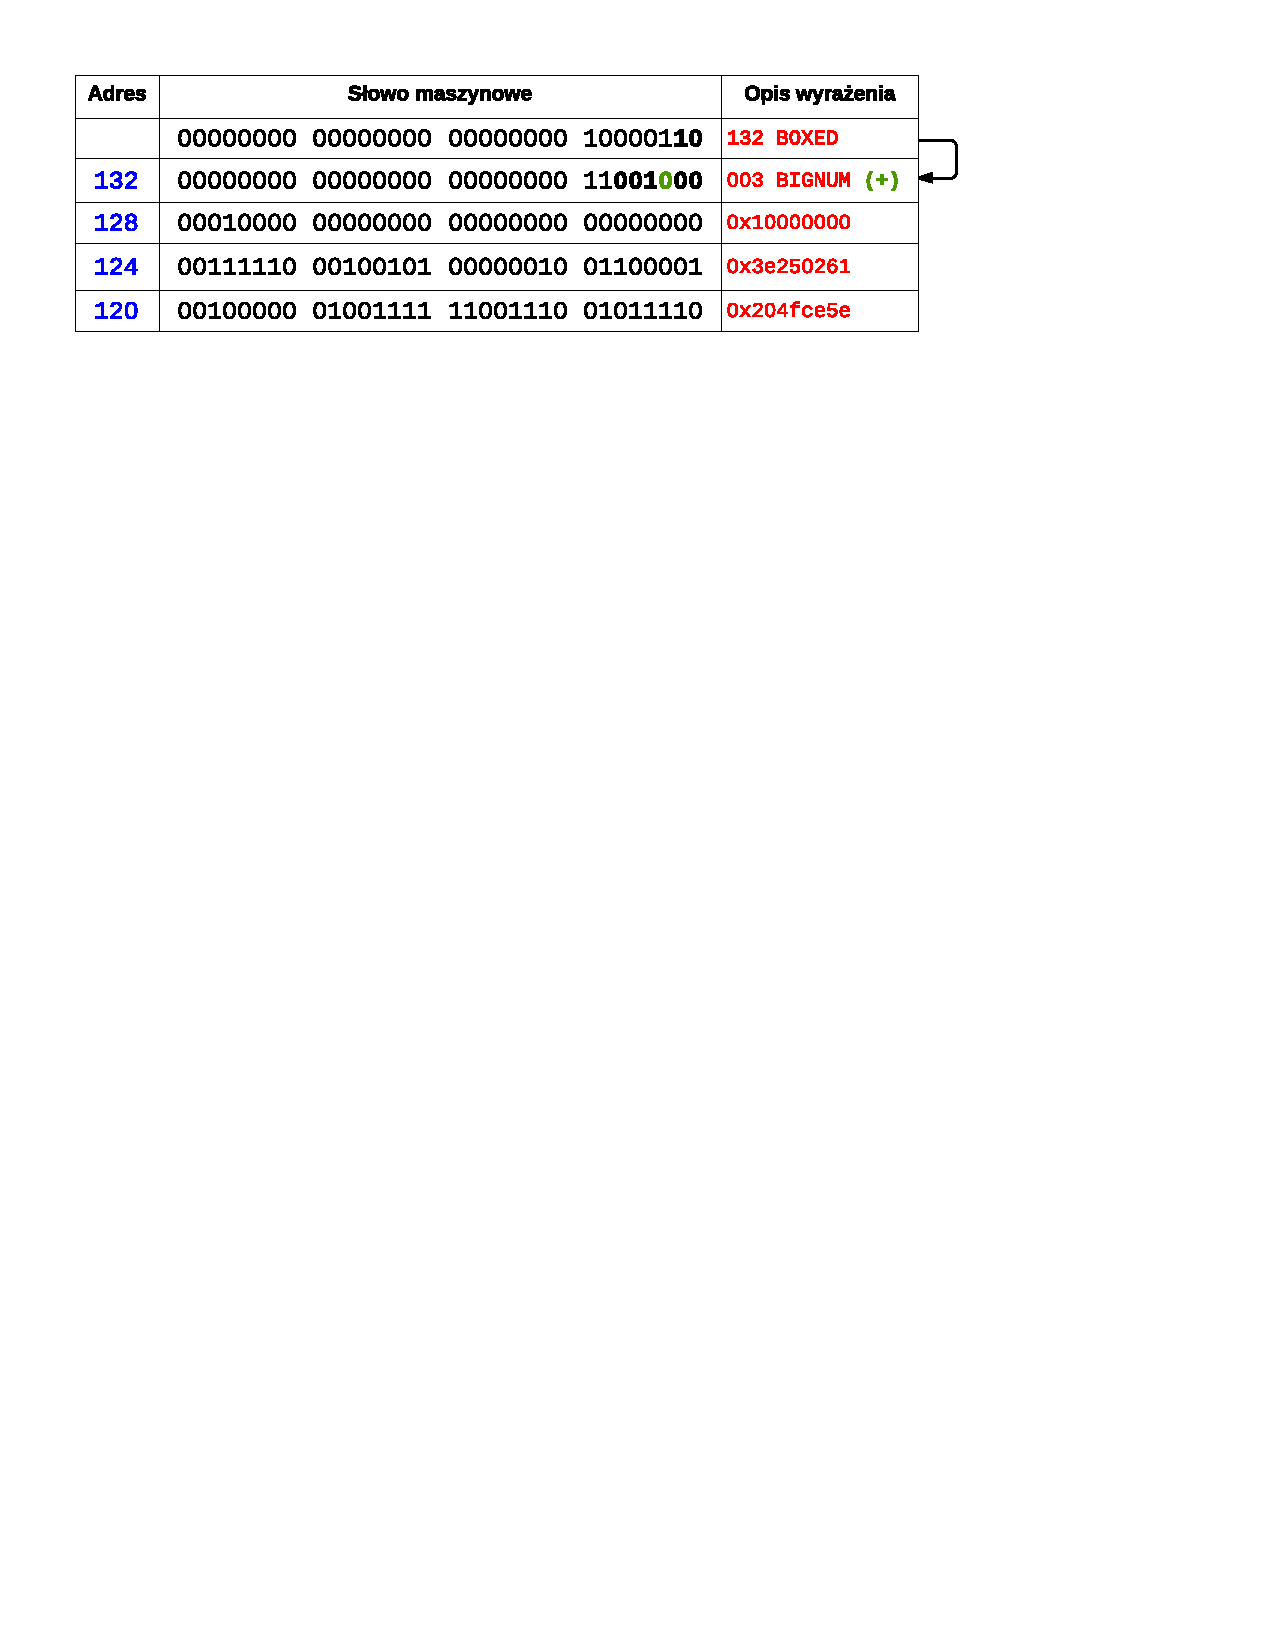
\includegraphics[scale=1, clip, trim=0 223mm 45mm 0]{bignum_on_heap}}
\caption{Przykład przechowywania dużej liczby na stercie procesu}
\label{fig:bignumonheap}
\end{figure}

\subsection{Niezaimplementowane typy danych}
\label{sub:typyNiezaimplementowane}

Typy danych dostępne w maszynie BEAM, które nie zostały zaimplementowane w pracy to:
\begin{itemize}
\item \textbf{lambdy} (tag \textbf{FUN}) - ten typ danych używany jest w komunikacji między węzłami wewnątrz klastra Erlanga, co nie jest aktualnie obsługiwane przez maszynę wirtualną, lambdy pojawiające się w kodzie źródłowym modułów reprezentowane są za pomocą funkcji lokalnych i nie potrzebują osobnego typu danych do poprawnego działania;
\item \textbf{referencje} (tag \textbf{REF}) - referencje z~założenia używane są do oznaczania wiadomości wysyłanych do innych węzłów z uruchomioną maszyną wirtualną a klastrowanie nie jest wspierane przez implementowaną maszynę wirtualną;
\item \textbf{porty} (tag \textbf{PORT}) - porty używane są do identyfikacji procesów uruchomionych w systemie operacyjnym poza maszyną wirtualną Erlanga, a do których delegowane są pewne operacje, wykonywane na poziomie systemu operacyjnego. Wykonanie tych operacji (jak np. operacje na plikach) z~założenia może zająć pewien dłuższy okres czasu, co mogłoby zakłócić harmonogramowanie procesów. Typ danych nie został zaimplementowany, gdyż w maszynie wirtualnej wszystkie operacje wykonywane na poziomie mikrojądra zostały zaimplementowane przy pomocy funkcji wbudowanych (por. \ref{sec:maszynaBIF});
\item \textbf{liczby zmiennoprzecinkowe} (tag \textbf{FLONUM}) - ten typ danych nie został zaimplementowany w~wersji maszyny opisywanej w pracy. Liczby zmiennoprzecinkowe rzadko wykorzystywane są w programowaniu urządzeń wbudowanych ze względu na bardzo duży narzut czasowych w przypadku mikrokontrolerów nie mających koprocesora (np. procesor ARM Cortex-M3 nie posiada FPU). M.in. z tego powodu do maszyny BEAM arytmetyka zmiennoprzecinkowa została dodana dopiero w wersji R8;
\item \textbf{binaria} (tagi \textbf{*\_BINARY}) - binarny typ danych włącznie ze wszystkimi operacjami dotyczącymi dopasowywania do nich zmiennych również nie został zaimplementowany w maszynie. Jest to funkcjonalność warta rozważenia w przypadku dalszej pracy nad maszyną ze względu na binarny charakter szeregowych interfejsów wejścia-wyjścia obsługiwanych przez mikrokontrolery. Podstawowe operacje na binariach do maszyny BEAM zostały dodane w wersji R7, bardziej zaawansowane były sukcesywnie dodawane od wersji R10.
\end{itemize}

%---------------------------------------------------------------------------
\section{Interpreter kodu maszynowego}
\label{sec:maszynaInterpreter}

Moduł opisany w niniejszym podrozdziale został zaimplementowany w pliku źródłowym \texttt{beam\_emu.c}.

\subsection{Maszyna stosowa a rejestrowa}
\label{sub:interpreterStosowa}

Spośród sposobów implementacji maszyny wirtualnej można wymienić dwa: maszynę stosową i~rejestrową.
Różnicę między tymi dwoma podejściami stanowi sposób przechowywania argumentów wywoływanej funkcji, miejsca zapisu wyniku jej wykonania oraz zmiennych tymczasowych przez nią używanych.

W przypadku maszyny stosowej dane te przechowywane są na stosie. Kolejne argumenty operacji umieszczane są na stosie za pomocą operacji \textbf{PUSH}, natomiast przed wykonaniem operacji zdejmowane są przez instrukcję \textbf{POP}. Instrukcje wykonywane przez maszynę wirtualną nie potrzebują zatem żadnych dodatkowych argumentów, gdyż te powinny być przed jej wywołaniem umieszczone na szczycie stosu, podobnie jak wynik zwrócony przez wykonaną instrukcję.

Z kolei w przypadku maszyny rejestrowej, powyższe informacje zapisywane są w zbiorze rejestrów.
Konsekwencją tego jest brak instrukcji manipulujących stosem w wykonywanym kodzie, co wpływa pozytywnie na szybkość działania interpretera kodu pośredniego.
Właściwe instrukcje wymagają jednak przekazania dodatkowych argumentów adresujących rejestry, w których znajdują się argumenty operacji i rejestr docelowy dla wyniku jej wykonania.
Efektem tego jest dłuższy zapis instrukcji w kodzie pośrednim niż w przypadku maszyny stosowej.
Dodatkowym atutem użycia rejestrów jest możliwość optymalizacji kodu polegającego na wyliczeniu i zapisaniu do rejestru pewnego pośredniego wyniku.
Wynik ten może następnie zostać wykorzystany przez kilka różnych instrukcji, zamiast wyliczania go od nowa przez każdą z nich.

Przykładami stosowych maszyn są maszyny języków takich jak Java czy .NET.
Z kolei przykładami maszyn rejestrowych są maszyny wirtualne języka Lua czy maszyna wirtualna Javy na system Android - Dalvik.

\subsection{Model interpretera}
\label{sub:interpreterModel}

Maszyna wirtualna języka Erlang (BEAM oraz maszyna zaimplementowana w pracy) jest również przykładem rejestrowej maszyny wirtualnej.

Interpreter korzysta z następujących rejestrów:
\begin{itemize}
\item rejestry \textbf{X\textsubscript{0}-X\textsubscript{255}} służące do przechowywania kolejnych argumentów z jakimi wywoływana jest funkcja, dodatkowo w rejestrze \textbf{X\textsubscript{0}} zapisywana jest wartość zwracana przez funkcję;
\item rejestry \textbf{Y} znajdujące się na stosie aktualnie uruchomionego procesu, służące do przechowywania zmiennych lokalnych;
\item rejestr \textbf{IP} przechowujący wskaźnik do aktualnie wykonywanej przez interpreter instrukcji;
\item rejestr \textbf{CP} przechowujacy adres powrotu - wskaźnik do instrukcji, którą interpreter powinien wykonać gdy nastąpi powrót z aktualnie wykonywanej funkcji.
\end{itemize}

Na listingu \ref{lis:maxS} zaprezentowany został przykładowy kod pośredni funkcji o arności 3, wyliczającej maksimum ze wszystkich jej argumentów, wykorzystujący do tego celu funkcję wbudowaną \texttt{erlang:max/2}. Wyjaśnienie działania poszczególnych operacji zostało zawarte w dodatku \ref{cha:operacjeBeam}.

\begin{lstlisting}[style=erlang, caption=Fragment kodu pośredniego liczącego maksimum z trzech wyrażeń modułu, label=lis:maxS]
{allocate,1,3}.
{move,{x,2},{y,0}}.
{call_ext,2,{extfunc,erlang,max,2}}.
{move,{y,0},{x,1}}.
{call_ext_last,2,{extfunc,erlang,max,2},1}.
\end{lstlisting}

Na rysunkach od \ref{fig:max1} do \ref{fig:max8} zaprezentowano zawartość rejestrów X (interpretera) i Y (na stosie procesu) po wykonaniu poszczególnych operacji kodu powyższego dla argumentów: \texttt{5,7,9}. Zapis \texttt{\{l,1\}} oznacza, że wskaźnik do instrukcji wskazuje na linię 1 z przykładu na listingu \ref{lis:maxS}, z kolei \texttt{erlang:max/2} oznacza, że wskaźnik do instrukcji wskazuje na początek tej funkcji wbudowanej. Przez zapis \texttt{CP} rozumiana jest wartość wskaźnika \textbf{CP} w chwili wywołania funkcji. 

Jak można zauważyć na rys. \ref{fig:max1} wszystkie trzy argumenty zostały umieszczone w rejestrach \textbf{X}: 0,~1~i~2. Instrukcja \texttt{\{allocate,1,3\}}, znajdująca się w pierwszej linii powoduje rozszerzenie stosu procesu o 2 wyrażenia, z czego na szczycie stosu umieszczany jest adres powrotu, z jakim została wywołana funkcja, zapisany pod wskaźnikiem \textbf{CP}.

W linii 2 (rys. \ref{fig:max3}) dokonane zostaje przeniesienie wyrażenia z rejestru \textbf{X\textsubscript{2}} do rejestru \textbf{Y\textsubscript{0}}, który jest pierwszym wyrażeniem na stosie poniżej jego szczytu.
Należy zauważyć, że pomimo wykorzystania stosu do zapisu zmiennych lokalnych, które nie zostaną zmodyfikowane pomiędzy wywołania funkcji, do operacji na nim nie wykorzystuje się operacji stosowych.
Nie należy zatem wiązać wykorzystania stosu procesu z faktem, że maszyna wirtualna jest maszyną stosową.

Przed wywołaniem funkcji \texttt{erlang:max/2} w linii 3, jako adres powrotu zostaje zapisana kolejna instrukcja w module, znajdująca się w linii 4. Argumentami wywoływanej funkcji są wartości znajdujące się w rejestrach \textbf{X\textsubscript{0}} i \textbf{X\textsubscript{1}}. Wywołana funkcja w momencie powrotu przepisuje wskaźnik powrotu (\textbf{CP}) na kolejną instrukcję do wykonania (\textbf{IP}). Wartość zwrócona z funkcji znajduje się w rejestrze \textbf{X\textsubscript{0}}. 

W linii 5 (rys. \ref{fig:max6}) wartość przechowywana na stosie zostaje przepisana do rejestru \textbf{X\textsubscript{1}}.
Drugie wywołanie funkcji \texttt{erlang:max/2} jest wywołaniem ogonowo-rekurencyjnym.
Dlatego też przykładowa funkcja odpowiedzialna jest za przywrócenie wskaźnika \textbf{CP} ze stosu i zwolnienie go jeszcze przed wywołaniem funkcji zewnętrznej. 
Wartość zwrócona z trójargumentowej funkcji znajduje się w rejestrze \textbf{X\textsubscript{0}}, a kolejna wykonana instrukcja będzie następująca po instrukcji, która ją wywołała.

\begin{figure}
\begin{multicols}{2}

\vspace{-4mm}
\begin{Figure}
 \centering
 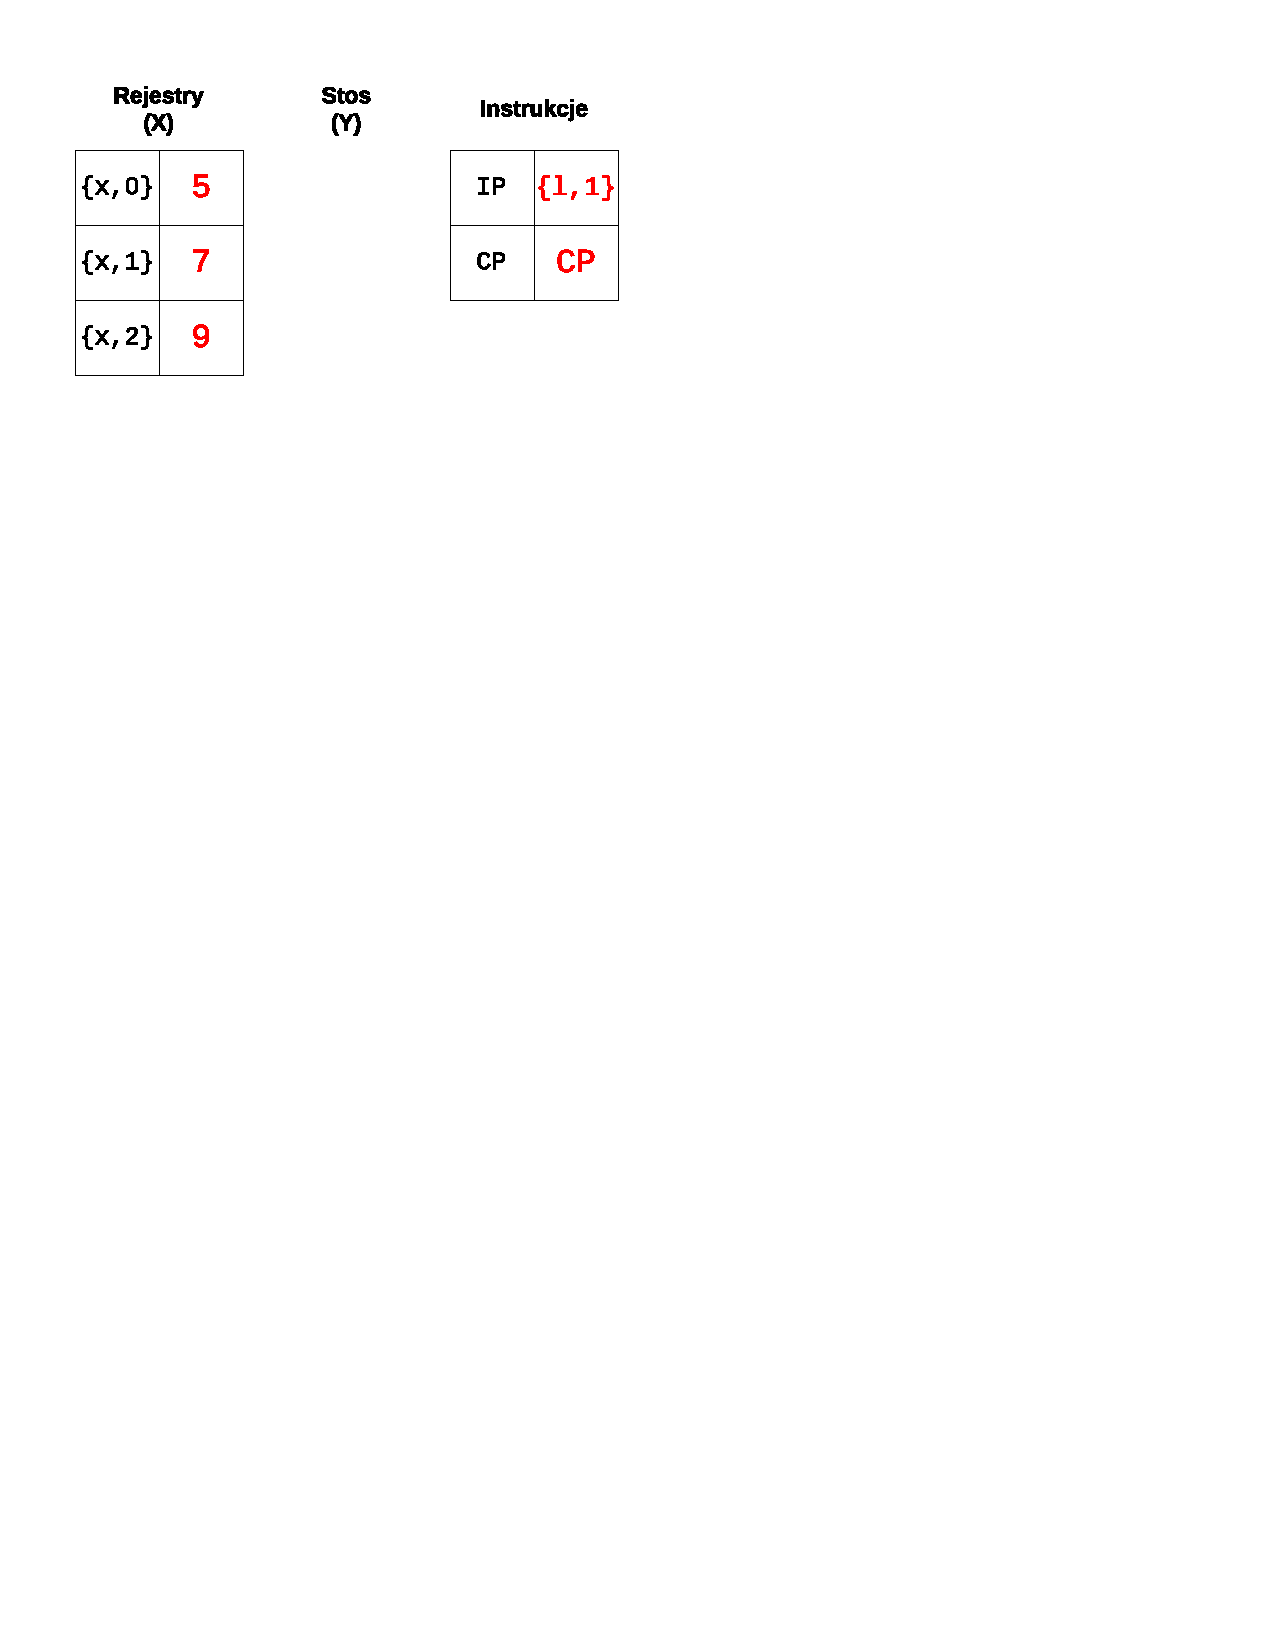
\includegraphics[scale=0.65, clip, trim=0 215mm 110mm 0]{interpreter_max_1}
\captionof{figure}{Rejestry przed wykonaniem instrukcji w linii 1}
\label{fig:max1}
\end{Figure}

\vspace{-4mm}
\begin{Figure}
 \centering
 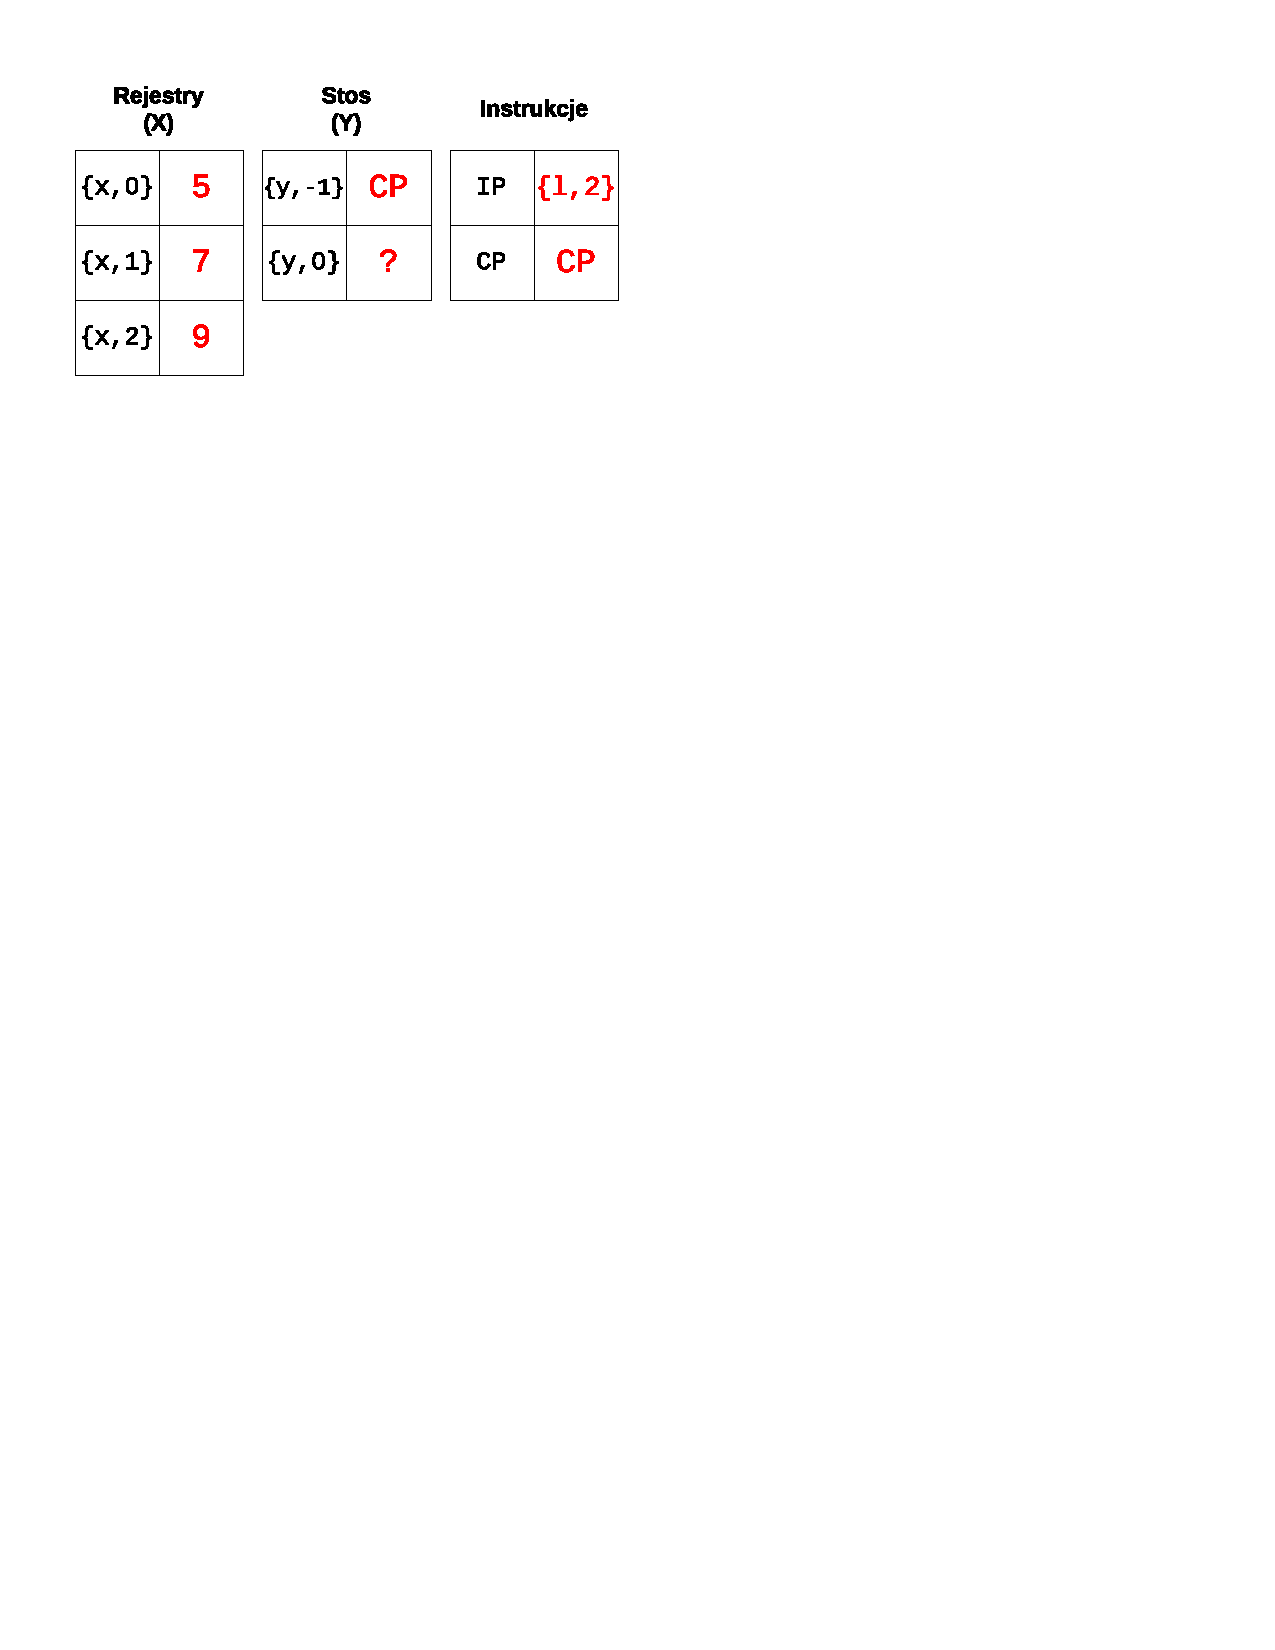
\includegraphics[scale=0.65, clip, trim=0 215mm 110mm 0]{interpreter_max_2}
\captionof{figure}{Rejestry przed wykonaniem instrukcji w linii 2}
\label{fig:max2}
\end{Figure}

\vspace{-4mm}
\begin{Figure}
 \centering
 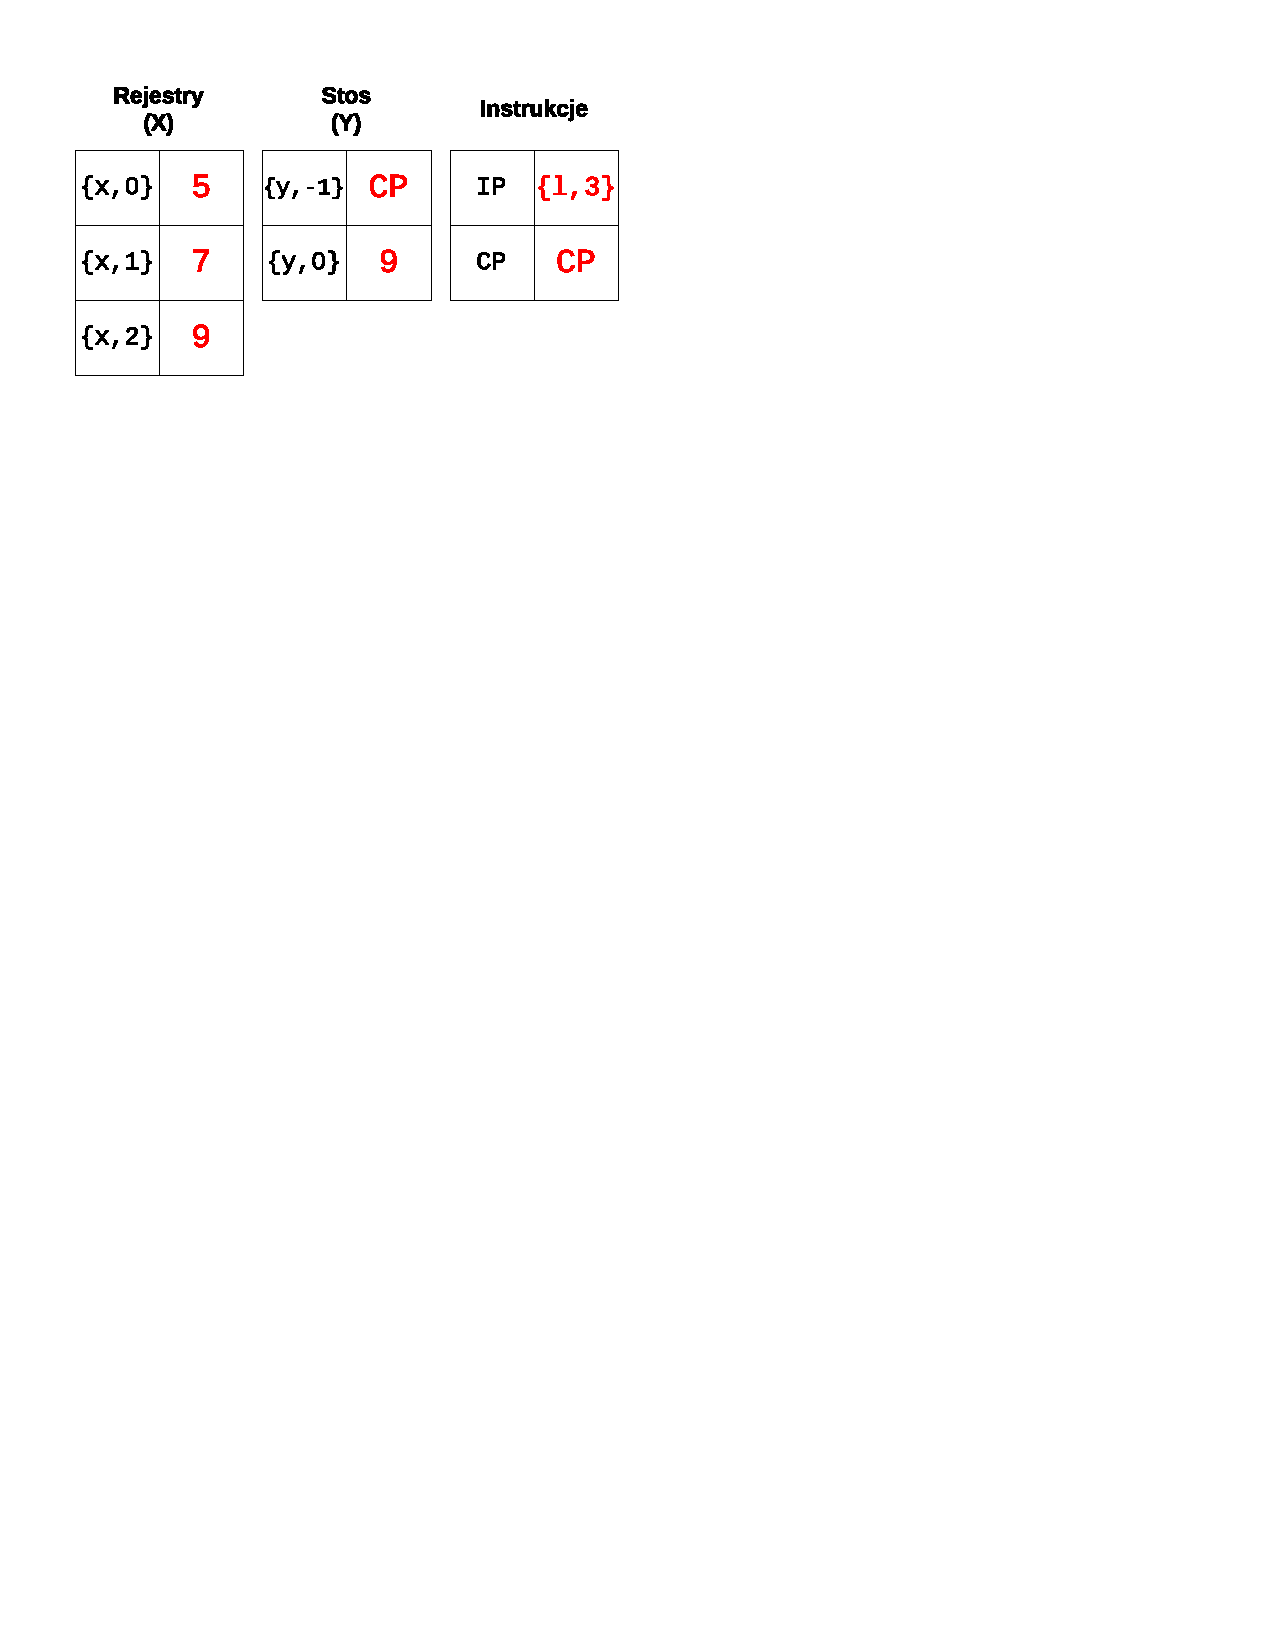
\includegraphics[scale=0.65, clip, trim=0 215mm 110mm 0]{interpreter_max_3}
\captionof{figure}{Rejestry przed wykonaniem instrukcji w linii 3}
\label{fig:max3}
\end{Figure}

\vspace{-4mm}
\begin{Figure}
 \centering
 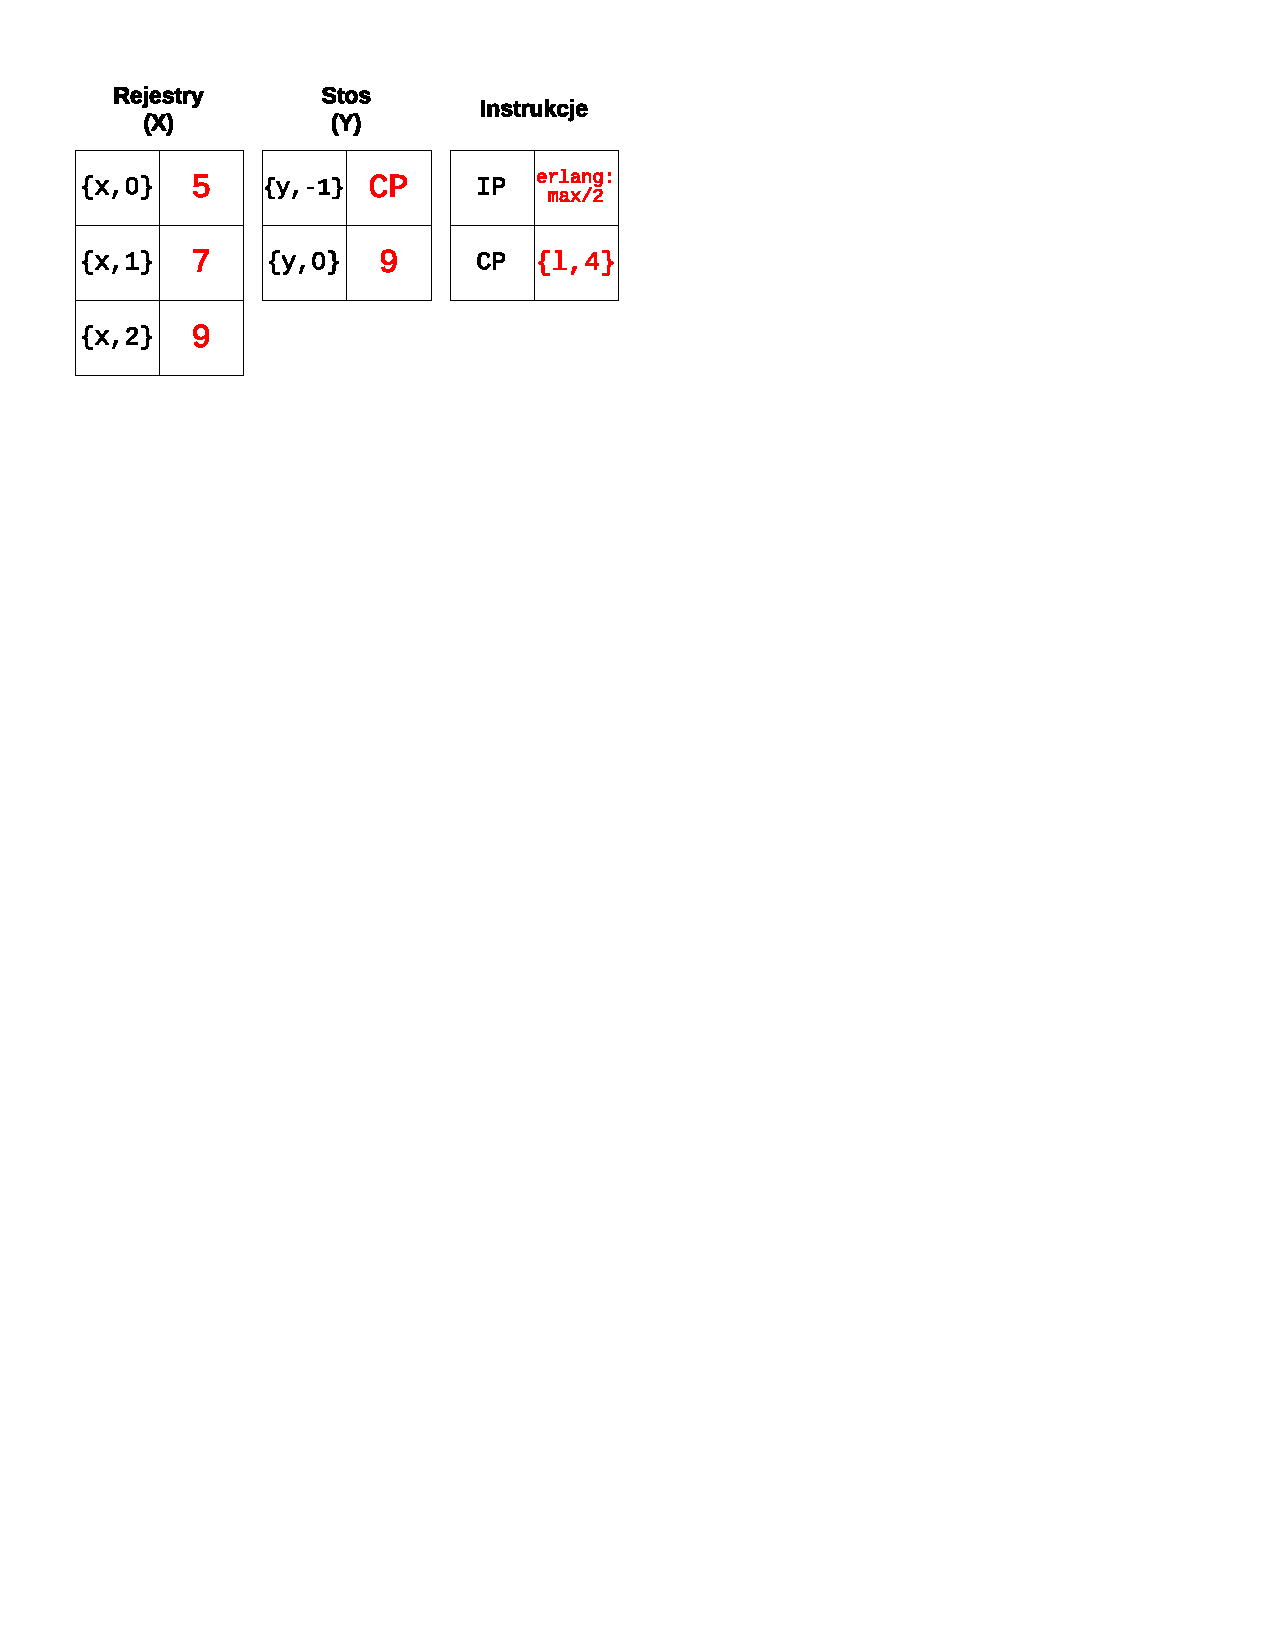
\includegraphics[scale=0.65, clip, trim=0 215mm 110mm 0]{interpreter_max_4}
\captionof{figure}{Rejestry przed wywołaniem funkcji w linii 3}
\label{fig:max4}
\end{Figure}

\vspace{-4mm}
\begin{Figure}
 \centering
 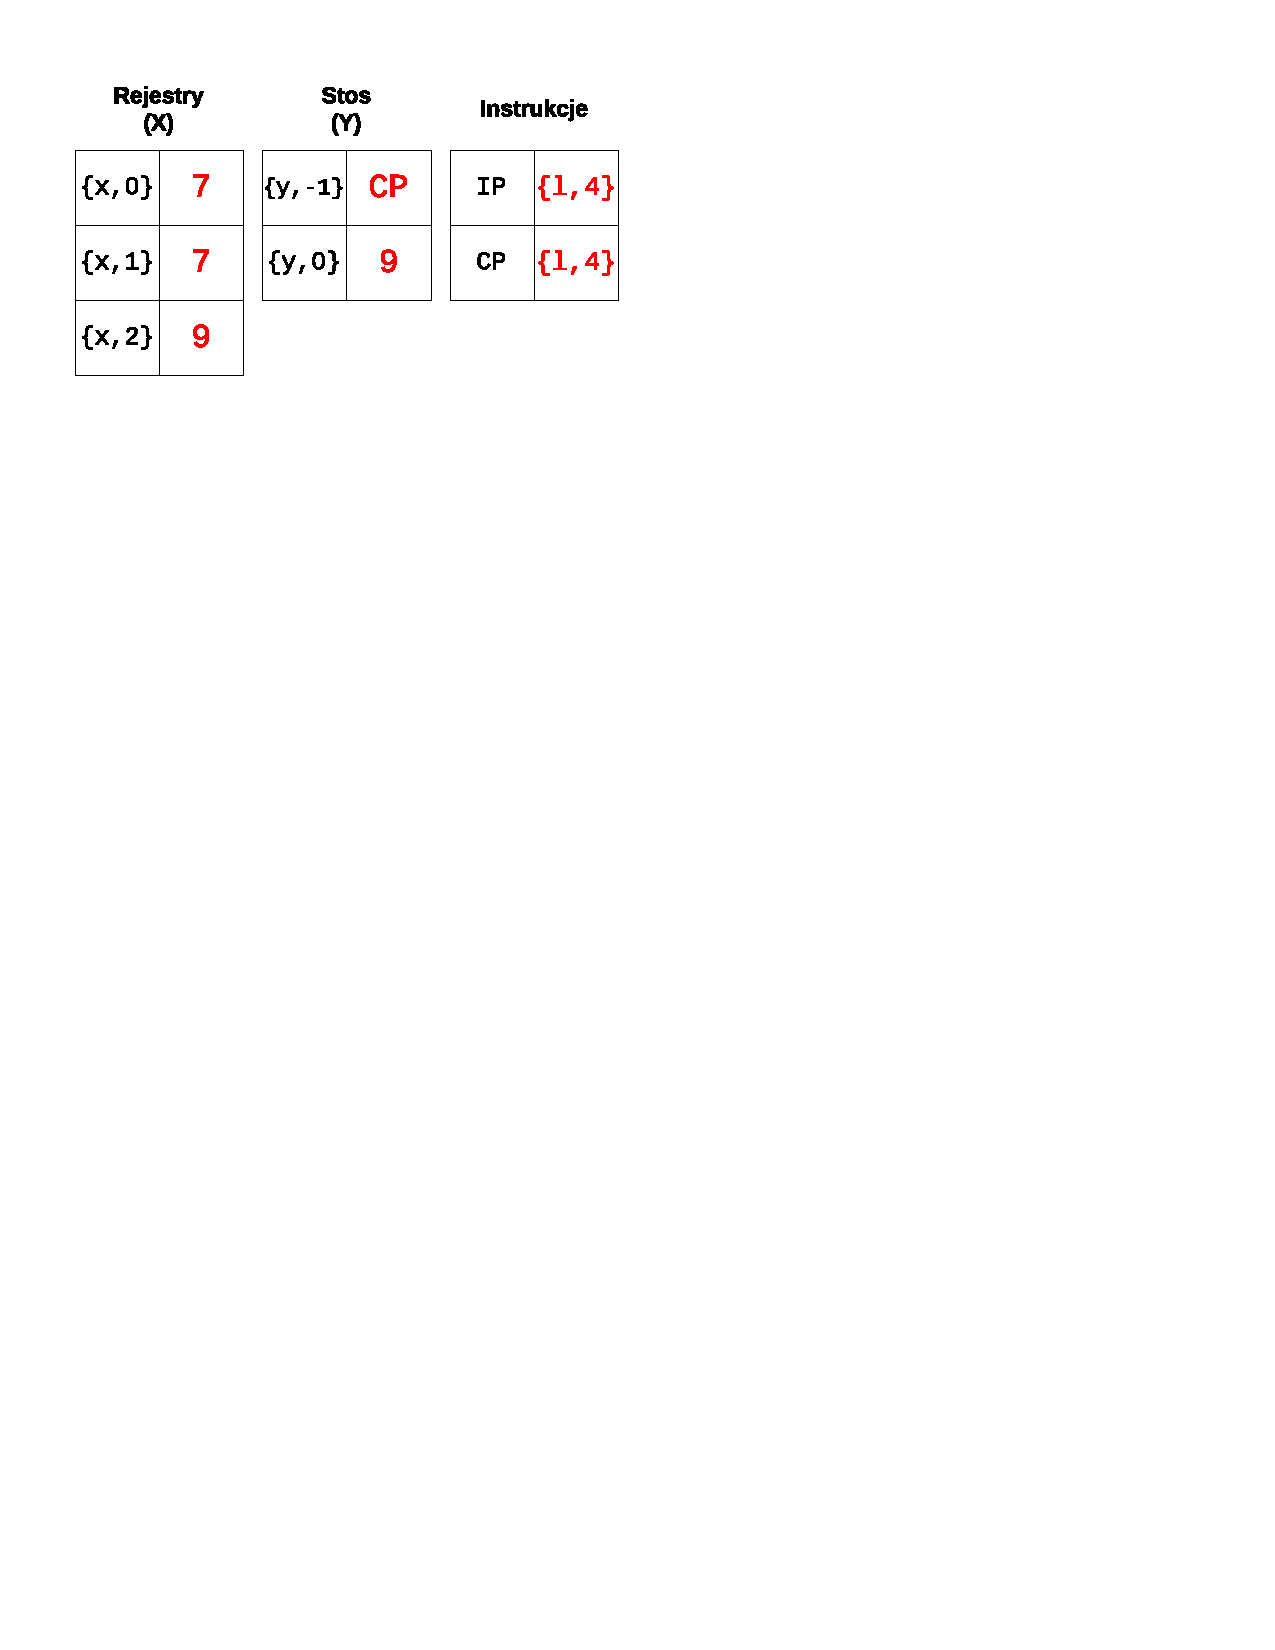
\includegraphics[scale=0.65, clip, trim=0 215mm 110mm 0]{interpreter_max_5}
\captionof{figure}{Rejestry przed wykonaniem instrukcji w linii 4}
\label{fig:max5}
\end{Figure}

\vspace{-4mm}
\begin{Figure}
 \centering
 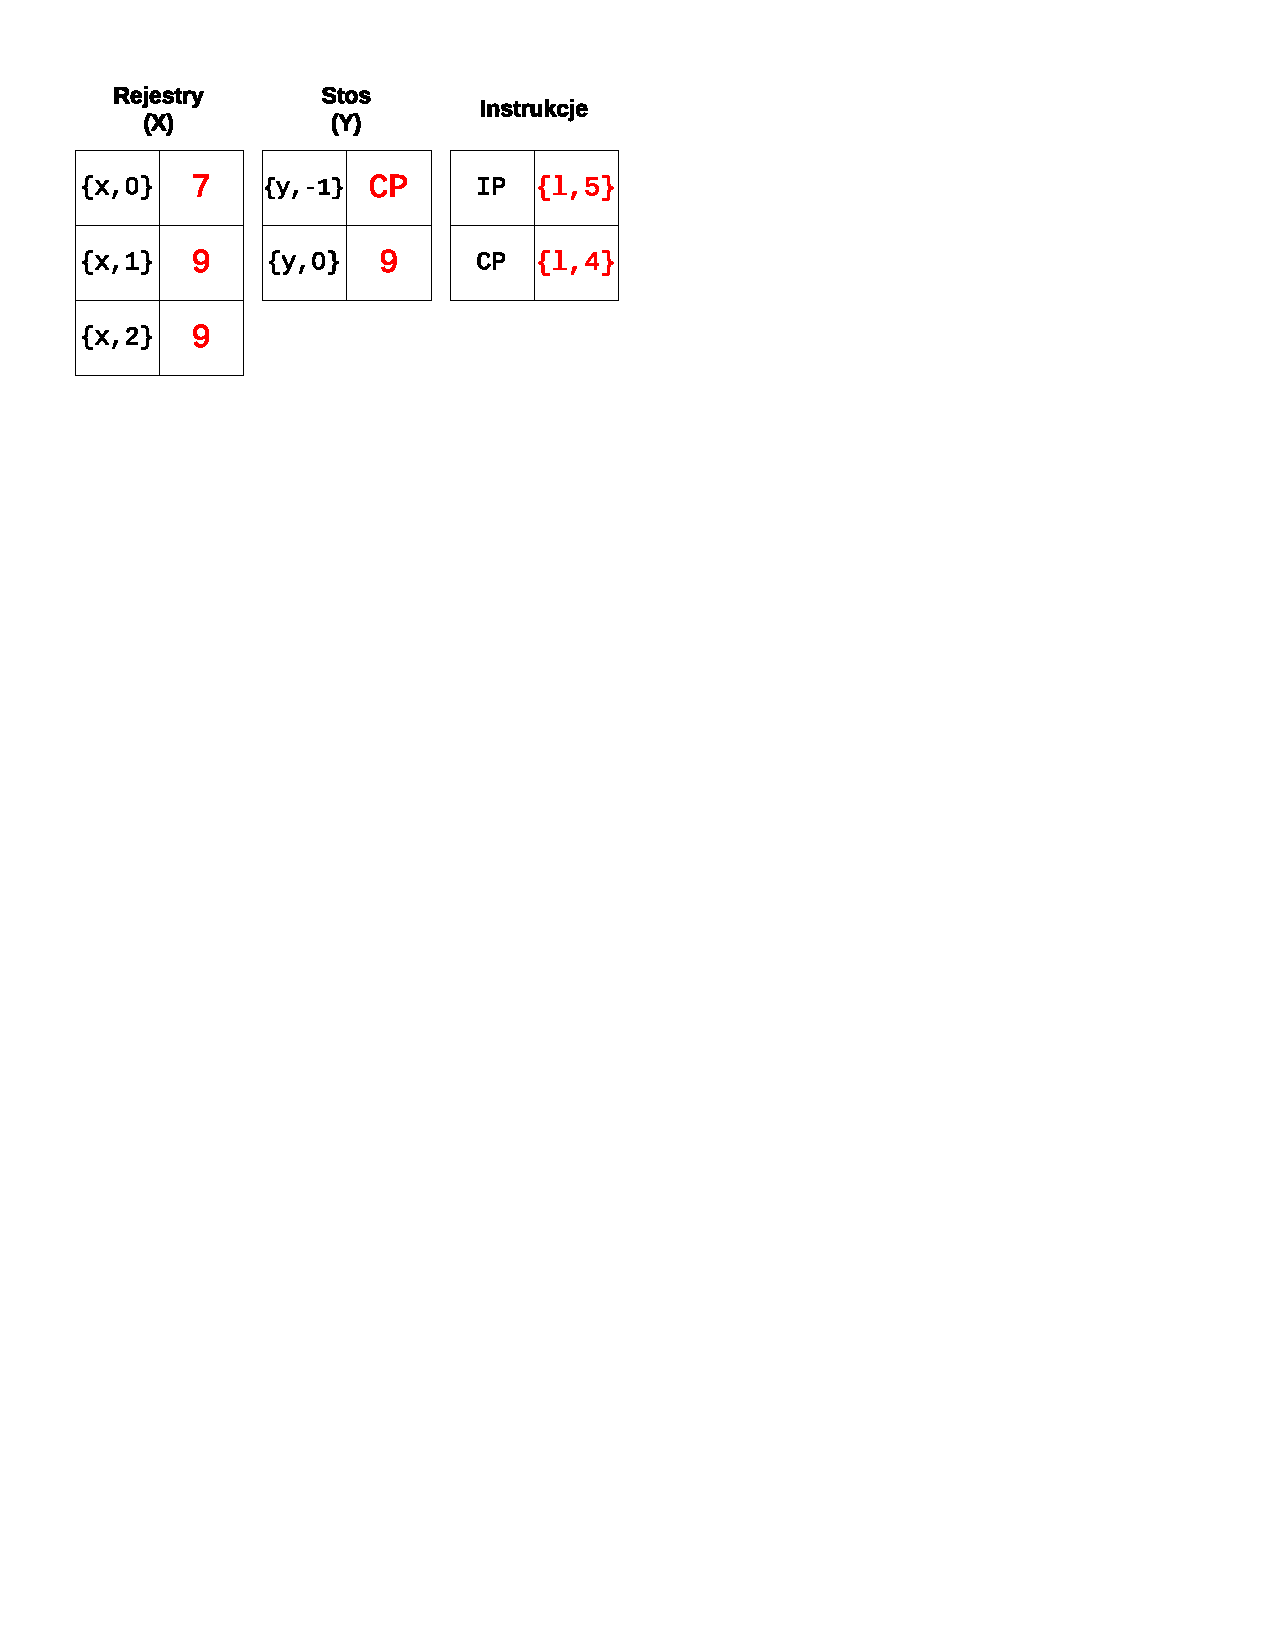
\includegraphics[scale=0.65, clip, trim=0 215mm 110mm 0]{interpreter_max_6}
\captionof{figure}{Rejestry przed wykonaniem instrukcji w linii 5}
\label{fig:max6}
\end{Figure}

\vspace{-4mm}
\begin{Figure}
 \centering
 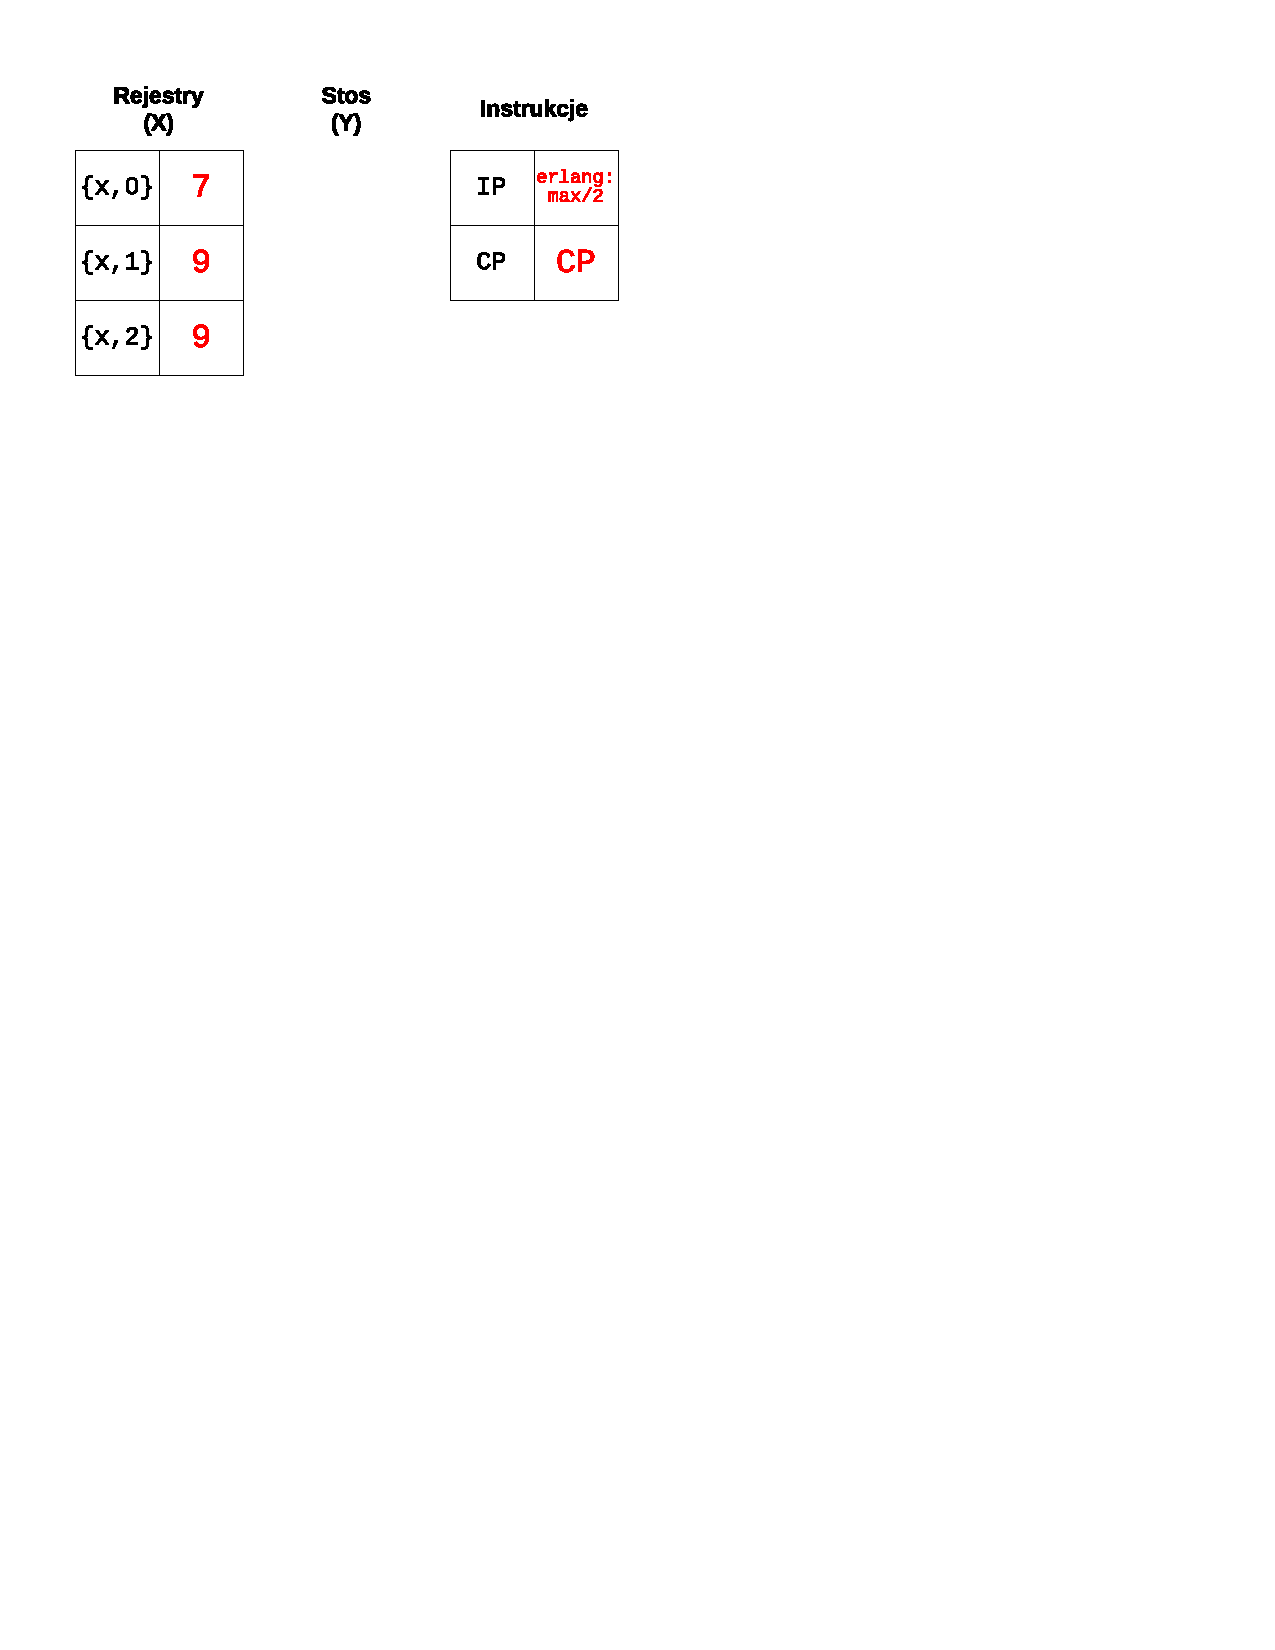
\includegraphics[scale=0.65, clip, trim=0 215mm 110mm 0]{interpreter_max_7}
\captionof{figure}{Rejestry przed wywołaniem funkcji w linii 5}
\label{fig:max7}
\end{Figure}

\vspace{-4mm}
\begin{Figure}
 \centering
 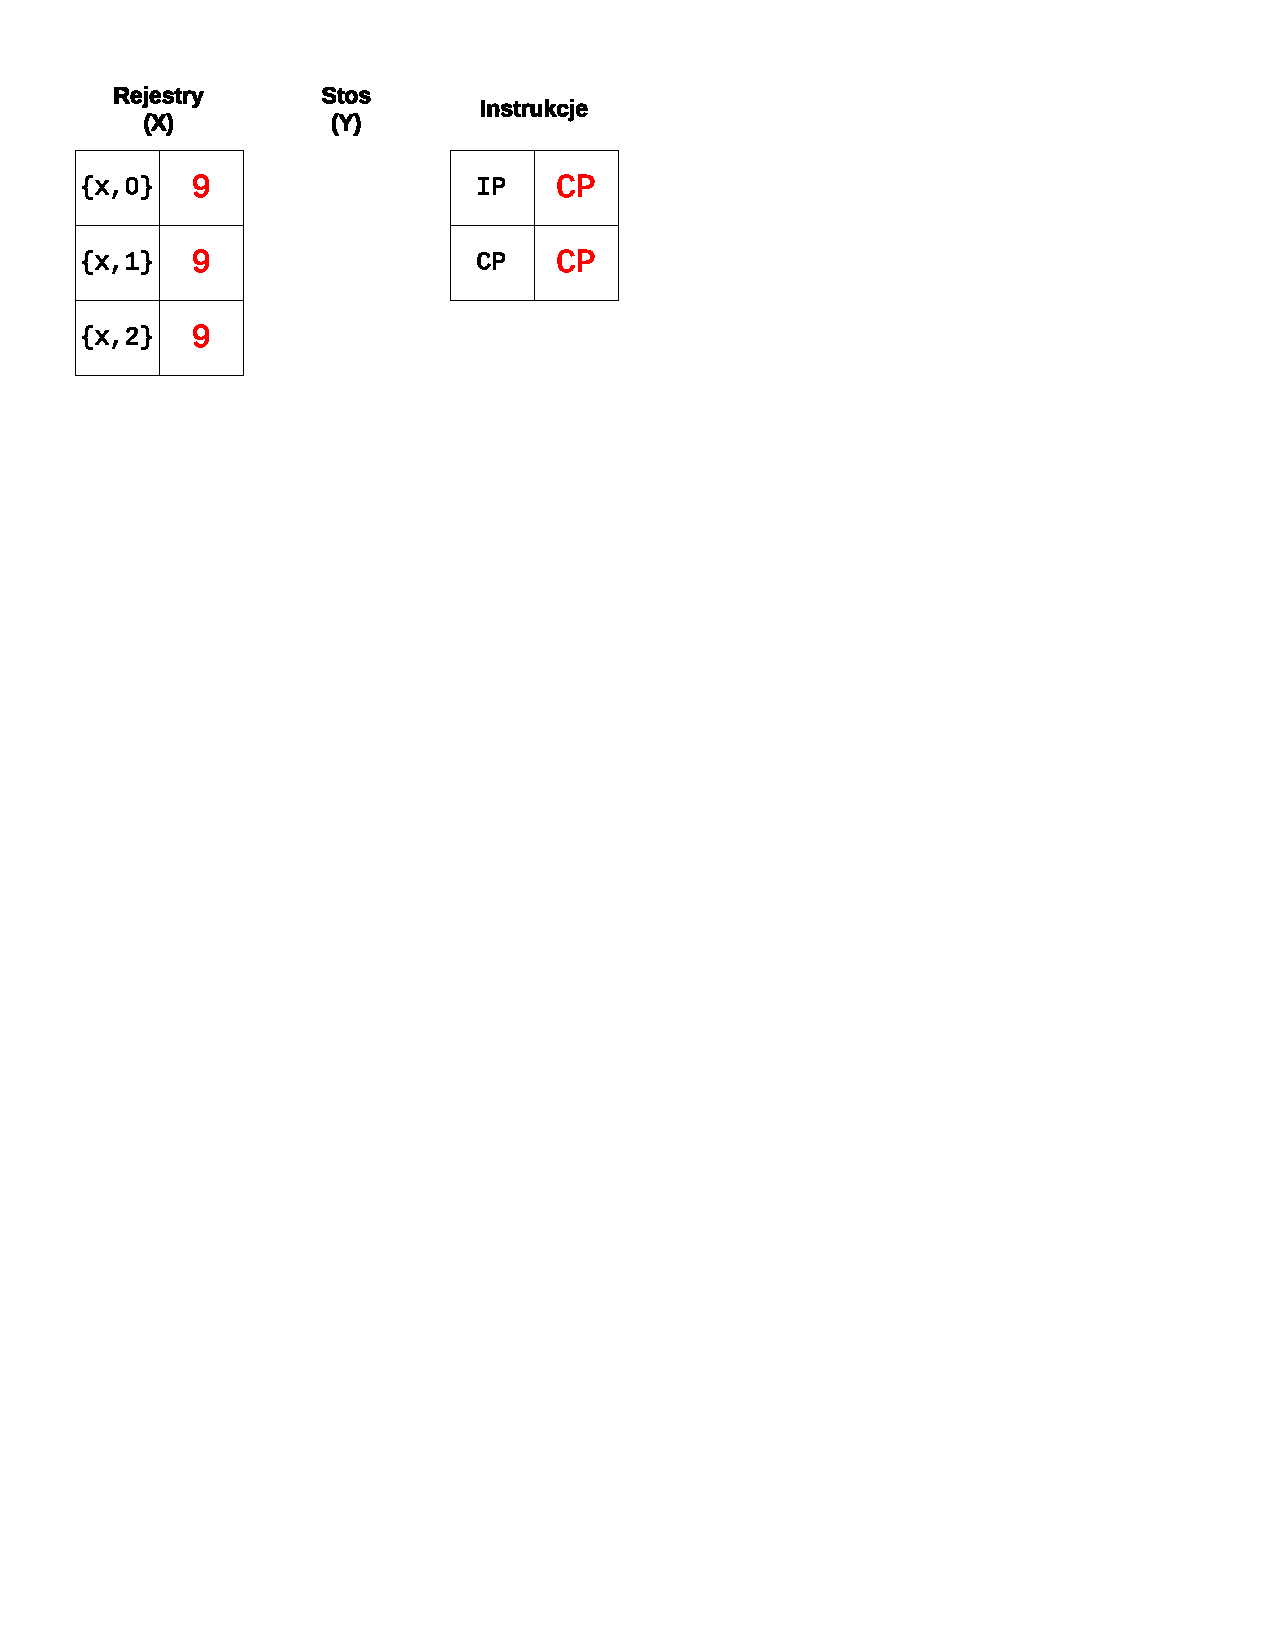
\includegraphics[scale=0.65, clip, trim=0 215mm 110mm 0]{interpreter_max_8}
\captionof{figure}{Rejestry po wykonaniu instrukcji w~linii 5, a zarazem i całej funkcji}
\label{fig:max8}
\end{Figure}
\end{multicols}
\end{figure}


%---------------------------------------------------------------------------
\section{Procesy}
\label{sec:maszynaProcesy}

%---------------------------------------------------------------------------
\section{Planista (\emph{scheduler})}
\label{sec:maszynaScheduler}

preemptive/cooperative, redukcje, wywłaszczenie, priorytety

%---------------------------------------------------------------------------
\section{Funkcje wbudowane (\emph{Built-In Functions})}
\label{sec:maszynaBIF}

\subsection{Funkcje ogólne (moduł \texttt{erlang})}
\label{sub:bifErlang}

\subsection{Listy (moduł \texttt{lists})}
\label{sub:bifLists}

\subsection{GPIO i obsługa przerwań (moduł \texttt{lpc\_gpio})}
\label{sub:bifGPIO}

\subsection{SPI (moduł \texttt{lpc\_spi})}
\label{sub:bifSPI}

%---------------------------------------------------------------------------
\section{\emph{Garbage collector}}
\label{sec:maszynaGC}

Cheney, długość sterty, rootset, gc

%---------------------------------------------------------------------------
\section{Mechanizmy zarządzania czasem}
\label{sec:maszynaTimer}

%---------------------------------------------------------------------------
\section{Podsumowanie różnic z maszyną BEAM}
\label{sec:maszynaPodsumowanie}

Na elementy, z których składa się maszyna wirtualna Erlanga można popatrzeć z punktu widzenia poszczególnych obszarów pamięci przez nią zajmowanych.

Do elementów tych należą:
\begin{itemize}
\item skompilowany kod wykonywalny modułów opisanych w niniejszym rozdziale;
\item tablice: atomów, eksportowanych funkcji, portów i procesów;
\item kolejki procesów i portów, na podstawie których \emph{scheduler} decyduje o wyborze kolejnego procesu do wykonania;
\item uruchomione procesy z informacjami kontrolnymi, kolejkami wiadomości i pamięcią do nich należącą;
\item załadowany kod pośredni modułów, który wykonywany jest w kontekście procesów;
\item globalna sterta, na której umieszczane są stałe wyrażenia pochodzące z plikami z modułów;
\item tablice ETS (\emph{Erlang Term Storage}) stanowiące w maszynie wirtualnej mutowalny obszar pamięci, w postaci bazy danych klucz-wartość;
\item sterta, na której przechowywane są dane typu binarnego, których długość wynosi przynajmniej 64 bajtów. Dane te mogą być współdzielone przez procesy, których liczba przechowywana jest przez licznik referencji, na którego podstawie \emph{garbage collector} zwalnia nieużywane już obszary pamięci.
\end{itemize}

Na rysunku \ref{fig:ertsmemory} zaprezentowany został powyższy podział, z uwzględnieniem elementów które posiada zarówno maszyna BEAM jak i maszyna zaimplementowana w pracy, które zostały oznaczone kolorem czarnym.
Kolorem niebieskim z kolei oznaczone zostały elementy, które nie zostały zaimplementowane w maszynie na system FreeRTOS.
Strzałki na diagramie przedstawiają fakt przechowywania wskaźników na elementy w jednym obszarze pamięci przed drugi.

\begin{figure}[h]
\centerline{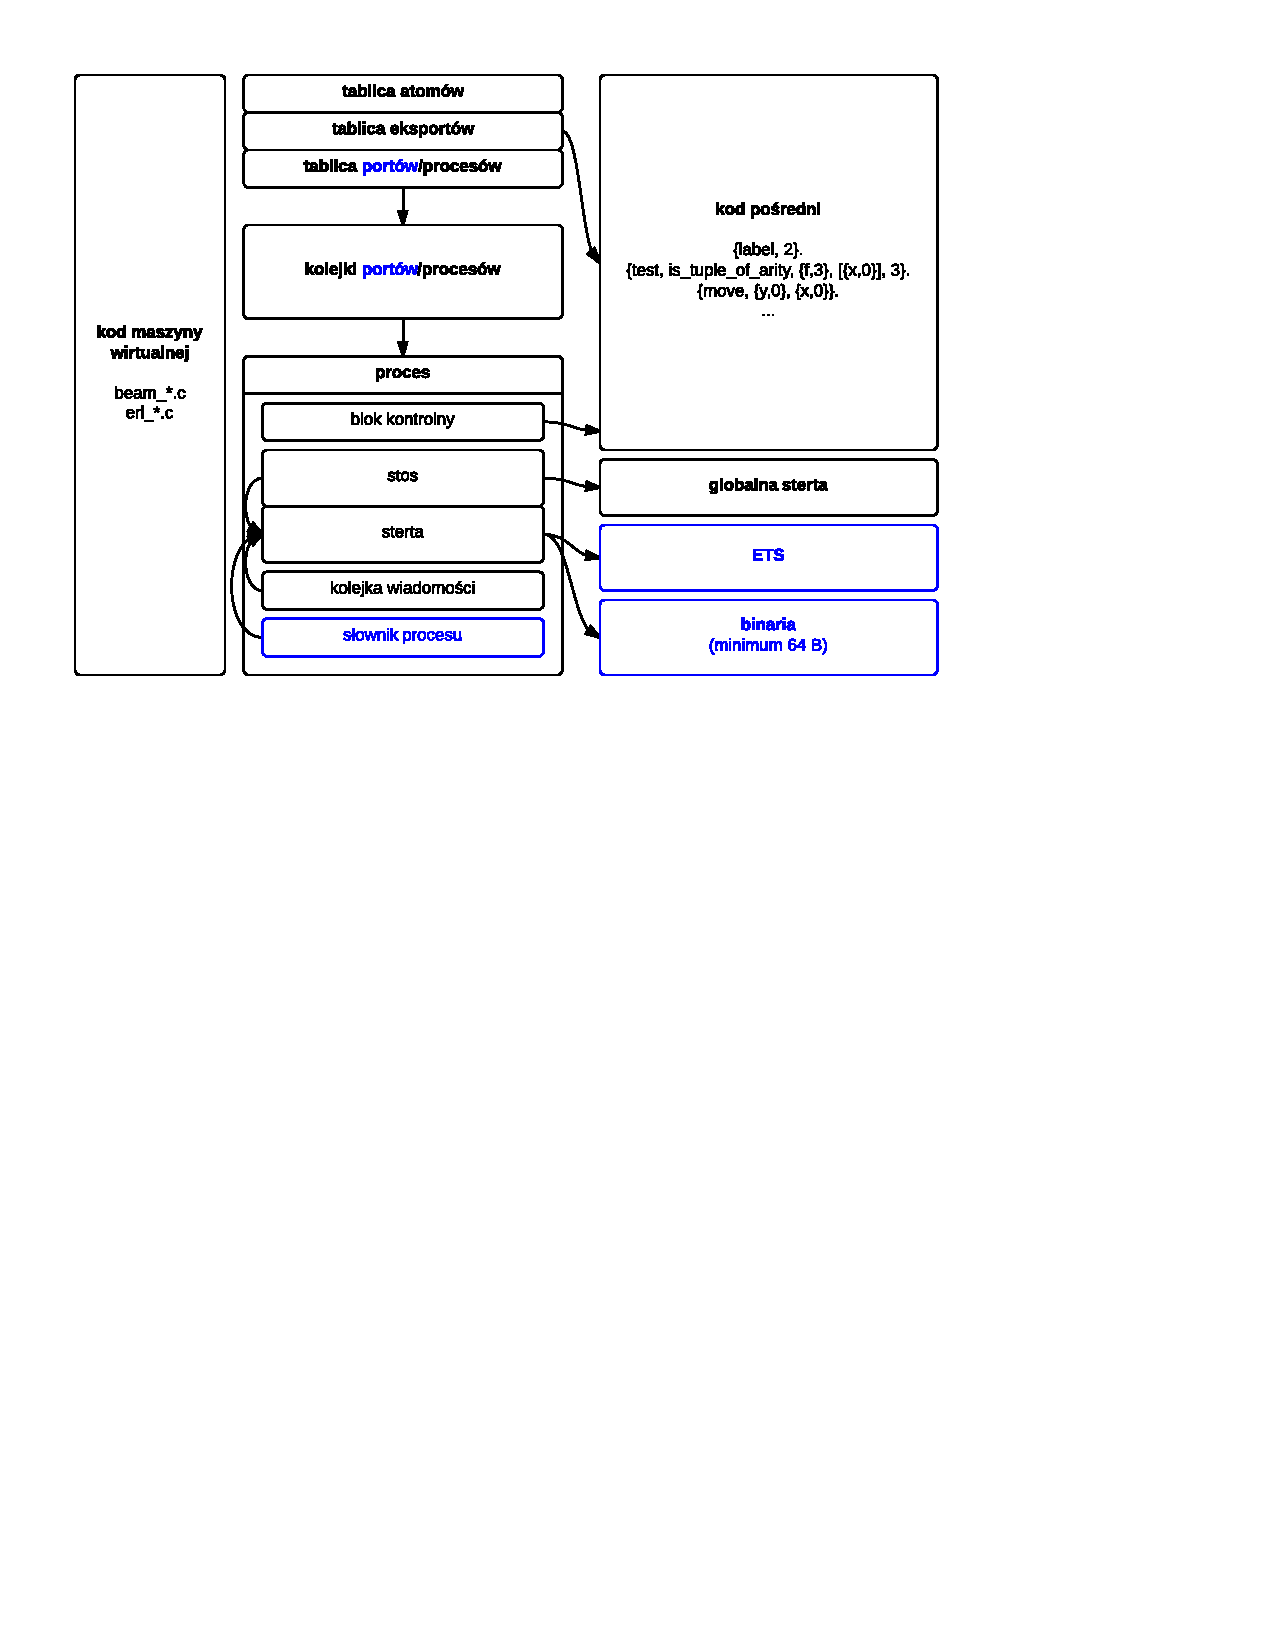
\includegraphics[scale=1, clip, trim=0 160mm 55mm 0]{erts_memory}}
\caption{Elementy maszyny wirtualnej Erlanga jako obszary pamięci.}
\label{fig:ertsmemory}
\end{figure}

Elementami, które nie zostały zaimplementowane w pracy są: tablice ETS oraz słownik procesu, których użycie nie jest konieczne do implementacji w pełni funkcjonalnych modułów w języku Erlang. Nie pozostały również zaimplementowane sterta binariów oraz tablice i kolejki portów, ze względu na niezaimplementowanie tych typów danych w maszynie.